\documentclass[]{book}
\usepackage{lmodern}
\usepackage{amssymb,amsmath}
\usepackage{ifxetex,ifluatex}
\usepackage{fixltx2e} % provides \textsubscript
\ifnum 0\ifxetex 1\fi\ifluatex 1\fi=0 % if pdftex
  \usepackage[T1]{fontenc}
  \usepackage[utf8]{inputenc}
\else % if luatex or xelatex
  \ifxetex
    \usepackage{mathspec}
  \else
    \usepackage{fontspec}
  \fi
  \defaultfontfeatures{Ligatures=TeX,Scale=MatchLowercase}
\fi
% use upquote if available, for straight quotes in verbatim environments
\IfFileExists{upquote.sty}{\usepackage{upquote}}{}
% use microtype if available
\IfFileExists{microtype.sty}{%
\usepackage{microtype}
\UseMicrotypeSet[protrusion]{basicmath} % disable protrusion for tt fonts
}{}
\usepackage{hyperref}
\hypersetup{unicode=true,
            pdftitle={User Guide for the MUX},
            pdfauthor={MultiplexÔ},
            pdfborder={0 0 0},
            breaklinks=true}
\urlstyle{same}  % don't use monospace font for urls
\usepackage{natbib}
\bibliographystyle{apalike}
\usepackage{longtable,booktabs}
\usepackage{graphicx,grffile}
\makeatletter
\def\maxwidth{\ifdim\Gin@nat@width>\linewidth\linewidth\else\Gin@nat@width\fi}
\def\maxheight{\ifdim\Gin@nat@height>\textheight\textheight\else\Gin@nat@height\fi}
\makeatother
% Scale images if necessary, so that they will not overflow the page
% margins by default, and it is still possible to overwrite the defaults
% using explicit options in \includegraphics[width, height, ...]{}
\setkeys{Gin}{width=\maxwidth,height=\maxheight,keepaspectratio}
\IfFileExists{parskip.sty}{%
\usepackage{parskip}
}{% else
\setlength{\parindent}{0pt}
\setlength{\parskip}{6pt plus 2pt minus 1pt}
}
\setlength{\emergencystretch}{3em}  % prevent overfull lines
\providecommand{\tightlist}{%
  \setlength{\itemsep}{0pt}\setlength{\parskip}{0pt}}
\setcounter{secnumdepth}{5}
% Redefines (sub)paragraphs to behave more like sections
\ifx\paragraph\undefined\else
\let\oldparagraph\paragraph
\renewcommand{\paragraph}[1]{\oldparagraph{#1}\mbox{}}
\fi
\ifx\subparagraph\undefined\else
\let\oldsubparagraph\subparagraph
\renewcommand{\subparagraph}[1]{\oldsubparagraph{#1}\mbox{}}
\fi

%%% Use protect on footnotes to avoid problems with footnotes in titles
\let\rmarkdownfootnote\footnote%
\def\footnote{\protect\rmarkdownfootnote}

%%% Change title format to be more compact
\usepackage{titling}

% Create subtitle command for use in maketitle
\providecommand{\subtitle}[1]{
  \posttitle{
    \begin{center}\large#1\end{center}
    }
}

\setlength{\droptitle}{-2em}

  \title{User Guide for the MUX}
    \pretitle{\vspace{\droptitle}\centering\huge}
  \posttitle{\par}
    \author{MultiplexÔ}
    \preauthor{\centering\large\emph}
  \postauthor{\par}
      \predate{\centering\large\emph}
  \postdate{\par}
    \date{2020-01-15}

\usepackage{booktabs}
\usepackage{amsthm}
\makeatletter
\def\thm@space@setup{%
  \thm@preskip=8pt plus 2pt minus 4pt
  \thm@postskip=\thm@preskip
}
\makeatother

\begin{document}
\maketitle

{
\setcounter{tocdepth}{1}
\tableofcontents
}
\hypertarget{reasons-for-the-mux}{%
\chapter{Reasons for the MUX}\label{reasons-for-the-mux}}

The first prototype of the system was built in 2010. The idea was that current water quality sensors are expensive and they are designed to be installed to obtain high frequency data at a particular station. In the field of hydrology, agrohydrology, ecohydrology, and limnology, to only name a few, there is a tight coupling between concentration variations in time and those in space. In other words, concentrations may vary by several folds within minutes and meters. To be able to track constituents and their fate over short distances (\textasciitilde{}\textless{} 50 m), one would ideally need not \emph{\textbf{one}} but \emph{\textbf{several}} sensors\ldots{} But then the price of such monitoring system would be prohibitive in the vast majority of cases. Not to mention that maintenance and chances of failure would be multiplied by the number of sensors deployed.

A more promising idea was to create a system that would be able to provide access to high enough frequency data for \emph{\textbf{multiple points}} in the vicinity of \emph{\textbf{one sensor}}. This solves the affordability problem as one sensor only is necessary, and it also solves the problem of multiplying maintenance on multiple sensors. Our solution is the MultiPlexed, MultiPoint Sampler or MPS, which we have now decided to call the \emph{MUX}, because it is just easier to say! And since you have the instrument with you now, you probably already have a pretty good idea of how it works.

\begin{figure}

{\centering 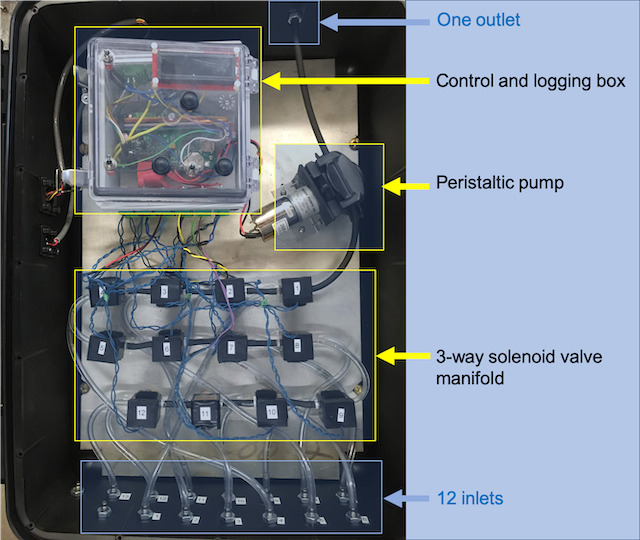
\includegraphics[width=0.8\linewidth]{pictures/MUXLayout} 

}

\caption{General Layout of the MUX, including a control box, a peristaltic pump, 12 3-way solenoid valves, 12 inlets, and one outlet}\label{fig:MUXLayout}
\end{figure}

Our solution is thus to bring water to the sensor, rather than the opposite. And once this idea became a promising solution, then expanding the `bringing of water to the sensor' to multiple points was a natural extension of the idea. All the MUX is, is a peristaltic pump for pumping and purging, a bunch of three-way solenoid valves (we chose 12 for now) that dictate which sampling point is activated, and a micro controller system to control and log all the MUX activities in synchrony with the sensor (Figure \ref{fig:MUXLayout}). The MUX sequentially pumps water from all the desired point to the sensor, and once all the points have been sampled, the sequence starts over again.

In theory, it is very simple. In practice, we have discovered that it takes a lot of attention to details to have a system that is robust enough to work over long periods of time reliably. We feel the version we have now is robust enough for others to use, although we are quite aware that there is still room for improvement, and we are dedicated to keep improving our system. We have published the details of the design and the performance of the MUX in \citeyearpar{Birgand2016-to}.

\hypertarget{the-versions-available}{%
\section{The versions available}\label{the-versions-available}}

Right now, we have three versions available. One specifically dedicated to work with the S::CAN field spectrophotometer called Spectro::lyser, one version that works with any sensor, and, a third version coupled with a synchronous syringe based sampler designed to sample rather small volumes of water at very low pumping rates (\textasciitilde{}around 1 ml/min).

\hypertarget{downloads}{%
\section{Downloads}\label{downloads}}

\begin{itemize}
\item
  Download the \href{https://francoisbirgand.github.io/Multiplexo/MUXManual.pdf}{SpectroMUX.pdf here}
\item
  Download the \href{https://francoisbirgand.github.io/Multiplexo/MUXManual.epub}{epub version here}
\end{itemize}

\hypertarget{intro}{%
\chapter{How to hook things together}\label{intro}}

\hypertarget{the-different-parts}{%
\section{The different parts}\label{the-different-parts}}

The version you have received works with a S::CAN spectro::lyser, a Con::nect box, a power supply cable connected between a battery or a AC to DC transformer, a 12V battery (+ solar panel for long term deployment) or a AC to DC transformer, a 6-pin and a 2-pin cables provided with the MUX, and the MUX itself. You need all these parts for things to work properly.

We use only 4 of the cables of the 6-pin cable. This cable is used to catch the cleaning or valve signal from the Spectro::lyser, which we later use trigger the MUX sampling sequence, and, to obtain the measurement data through the RS485 connection and communication protocol.

We use the 2-pin cable to power the MUX. Honestly, we could have used the 6-pin cable and use all 6 cable to do, power, cleaning signal, and the data transfer, but by default, we like to keep a cable dedicated to power.

\hypertarget{connecting-with-the-connect-box}{%
\section{Connecting with the Con::nect Box}\label{connecting-with-the-connect-box}}

All wires to the MUX are connected to the Con::nect Box. To use with the MUX, we use the left panel of the Con::nect Box (Figure \ref{fig:connectboxfull}).

\begin{figure}

{\centering 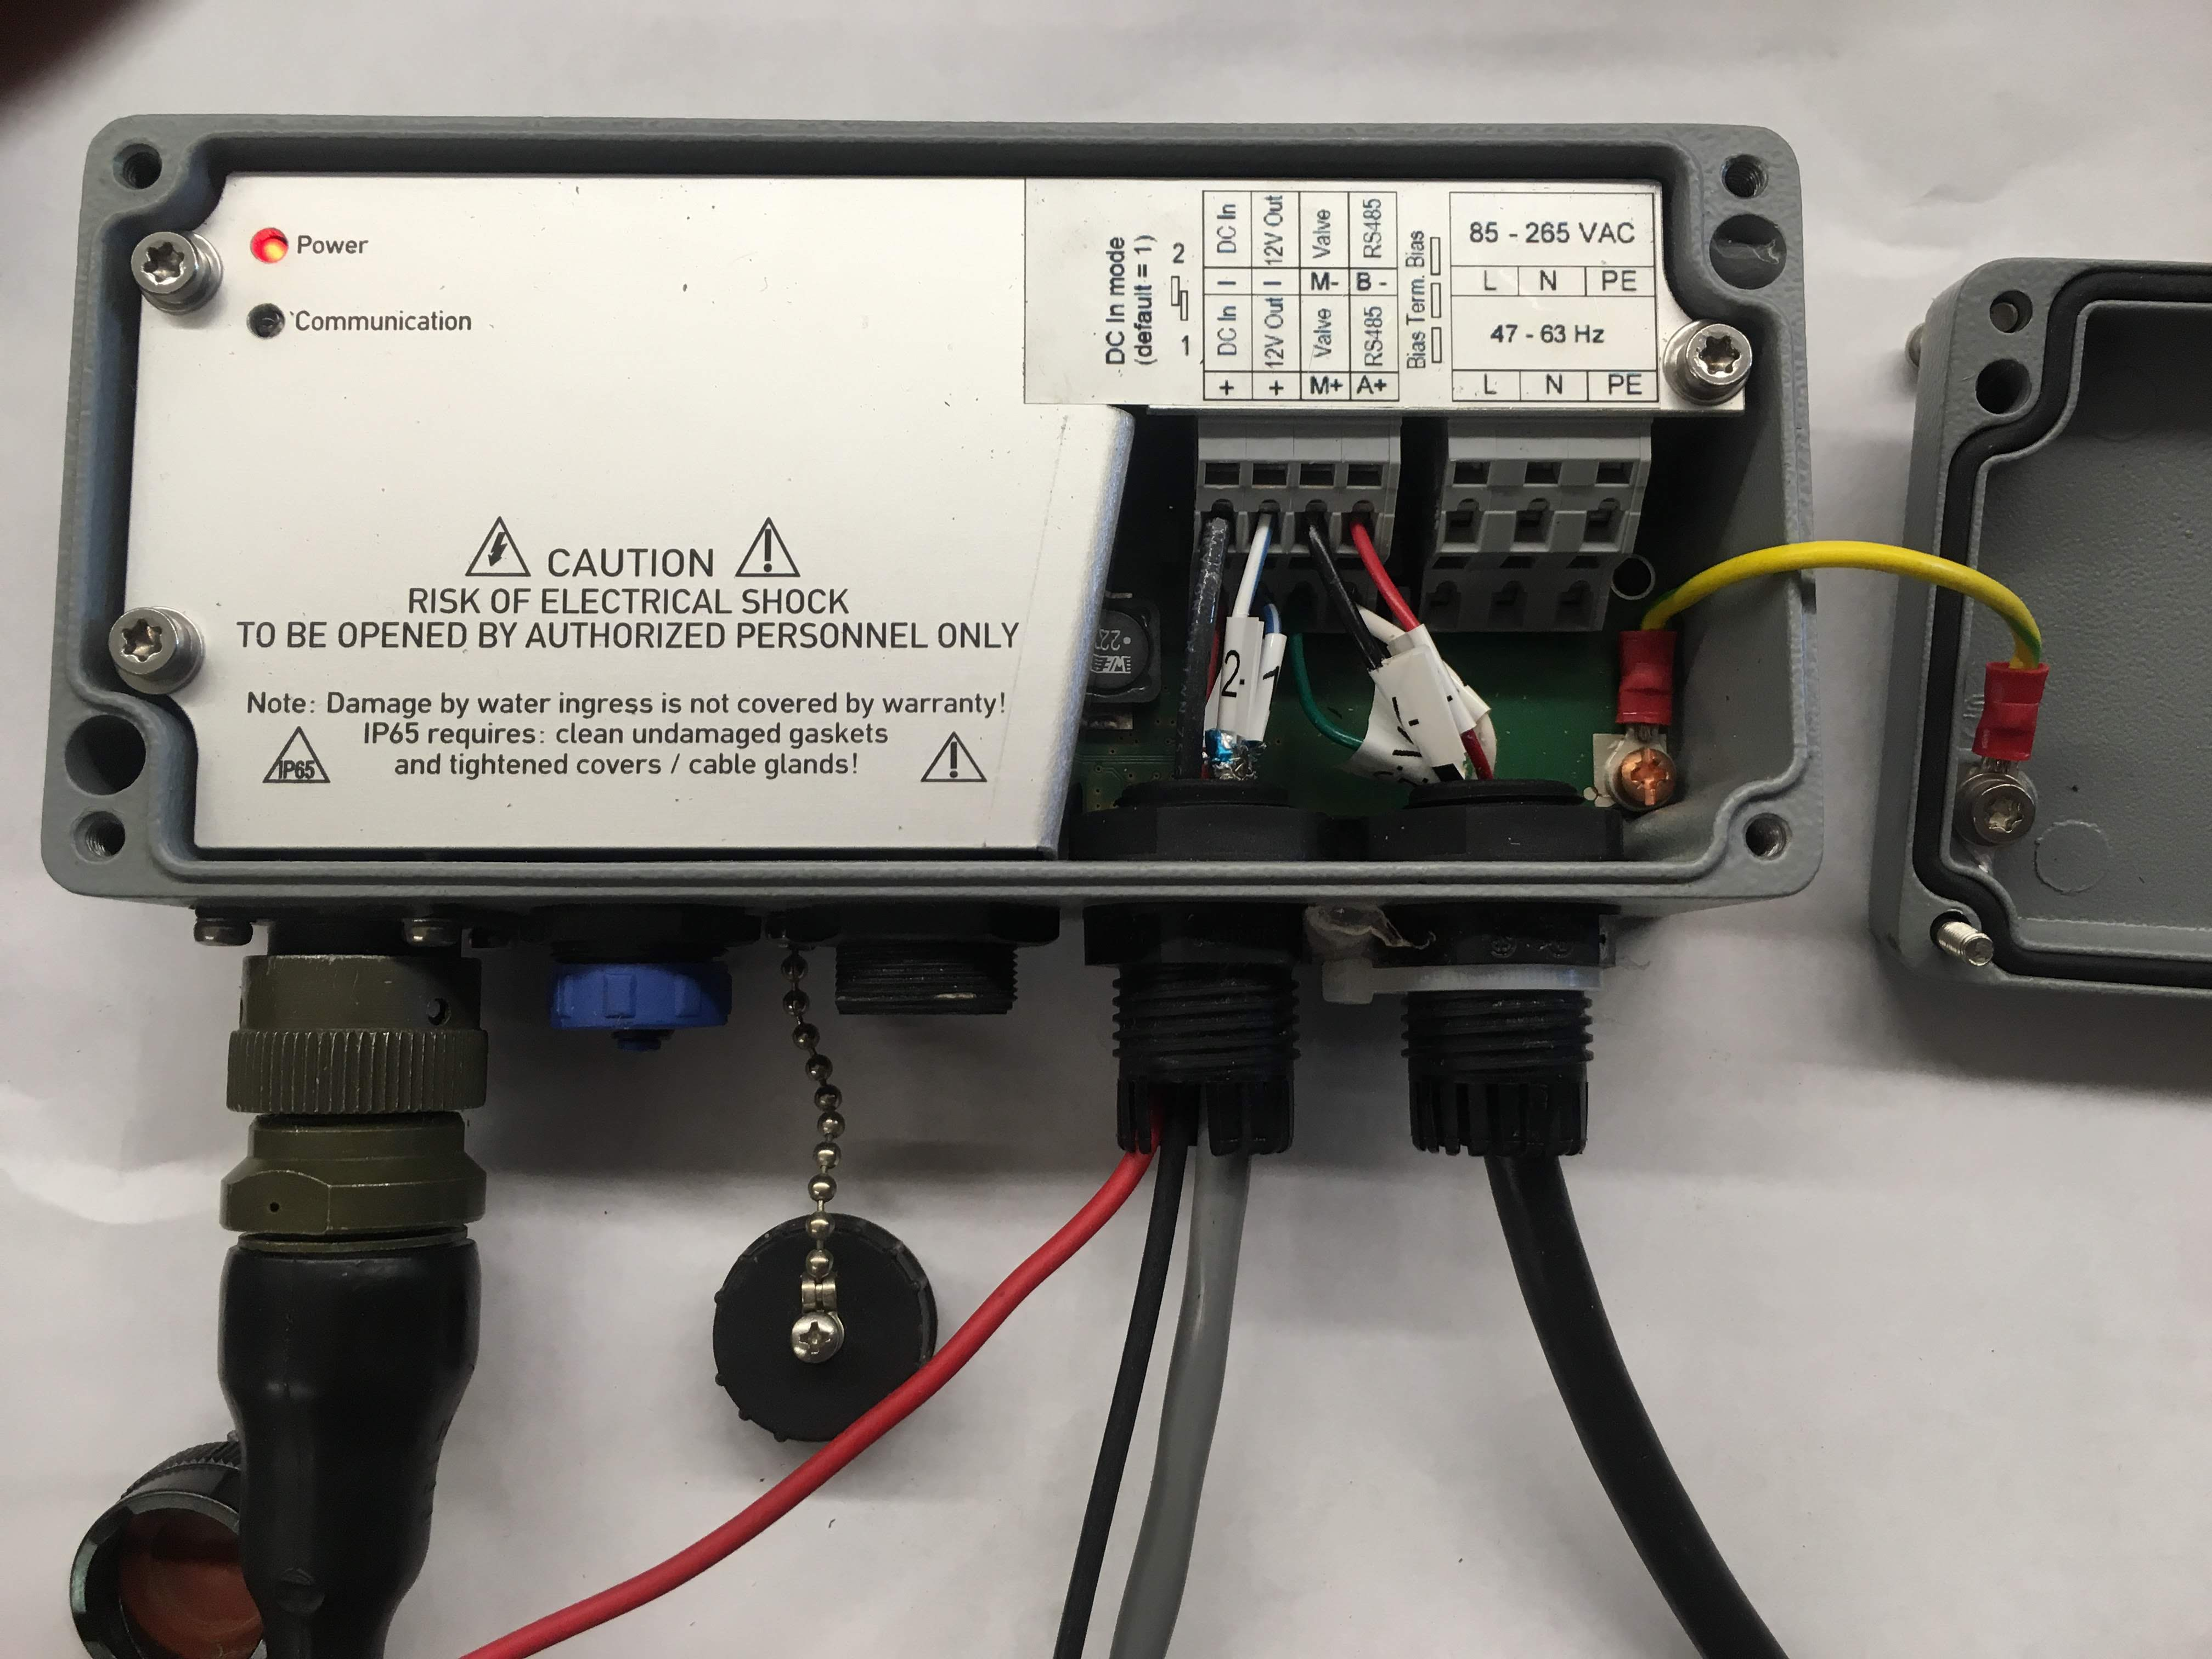
\includegraphics[width=0.7\linewidth]{pictures/ConnectBoxFull} 

}

\caption{picture of the connecting capabilities inside the Con::nect Box}\label{fig:connectboxfull}
\end{figure}

\hypertarget{powering-the-connect-box}{%
\subsection{Powering the Con::nect Box}\label{powering-the-connect-box}}

At the most left side, the user connects the wires either connected a 12V battery, or to an AC to DC adapter, which delivers 12V. This is referred to as `DC In' on the Con::nect Box label (Figure \ref{fig:connectboxfull}). By convention, the positive wire is normally red and the negative wire, black. The black or negative wire is at the top or right of the label, and the red or positive wire is at the bottom (not really visible on Figure \ref{fig:connectboxfull}). Make sure you use at least 14 gauge for these wires, to be on the safe side.

All the Con::nect Box connections are done using spring-loaded terminal. You need to use a fine screwdriver and insert it on the top part of the terminal (yellow arrows on Figure \ref{fig:SpringLoadedTerminal}), gently push or rotate down to open the spring-loaded connection located below (magenta arrows on Figure \ref{fig:SpringLoadedTerminal}). While open, insert the wire as deep as you can to obtain the best and secure connection, while still leaving the plastic sheathing out. Make sure the free wires are not longer than 4 mm, however, otherwise free wires will be stay out and that is not ideal. After you have inserted the wires, make sure you pull on the wire. If it comes out easily, do it again until it is hard to pull on it. Also, always insert the bottom wires first.

\begin{figure}

{\centering 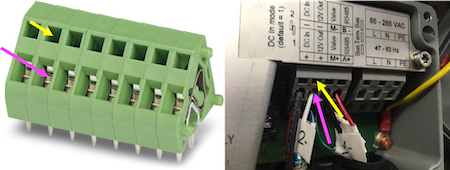
\includegraphics[width=0.9\linewidth]{pictures/SpringLoadedConnections} 

}

\caption{Spring-loaded connections for the Con::nect Box}\label{fig:SpringLoadedTerminal}
\end{figure}

The three other connection types include `12V out', `Valve', and `RS485', and we use all three with the MUX.

\hypertarget{powering-the-mux}{%
\subsection{Powering the MUX}\label{powering-the-mux}}

The MUX is powered by the `12V out' connection. The Con::nect Box provides a source of 12V power to other instruments that might be connected to it and we are taking advantage of this system to power the MUX. For that you will use the 2-pin cable as illustrated in Figure \ref{fig:2-pin-cable} below.

\begin{figure}

{\centering 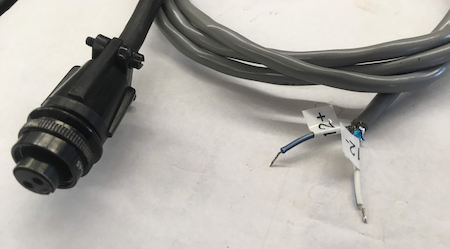
\includegraphics[width=0.7\linewidth]{pictures/2-pin-cable} 

}

\caption{2-pin cable to provide 12V DC power to the MUX, with the blue wire as '+' and the white wire as '-'}\label{fig:2-pin-cable}
\end{figure}

The blue wire corresponds to the positive or ``+'' and the white wire corresponds to the negative or `-'. As illustrated in Figure \ref{fig:ConnectBox1}, insert the blue ``+'' wire at the bottom or left connection, and the white ``-'' wire at the top or right connection of the `12V out' terminal.

\begin{figure}

{\centering 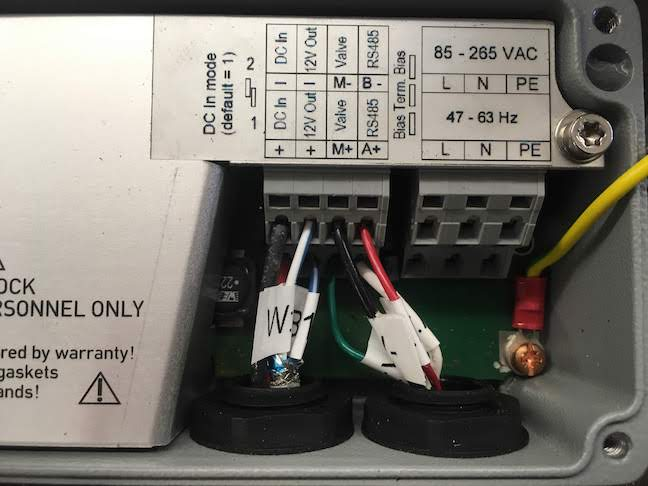
\includegraphics[width=0.7\linewidth]{pictures/ConnectBox1} 

}

\caption{2-pin cable to provide 12V DC power to the MUX, with the blue wire as '+' and the white wire as '-'}\label{fig:ConnectBox1}
\end{figure}

\hypertarget{connections-to-trigger-the-mux}{%
\subsection{Connections to Trigger the MUX}\label{connections-to-trigger-the-mux}}

The Con::nect box has a connection through which it can send a 12V signal for a specified amount of time. Actually, it is the spectro::lyser that sends the 12V. Originally, this was used to open an air valve to send a burst of compressed air to clean up the optics. Later it has been used to activate an automatic brush, also to clean the optics. We are using this feature to start a sampling sequence from the MUX. When at idle, the MUX is listening to such a 12V signal, and upon receiving this signal the MUX starts its sampling sequence.

For this we use the black and green wires of the 6-pin cable (Figure \ref{fig:6-pin-cable}).

\begin{figure}

{\centering 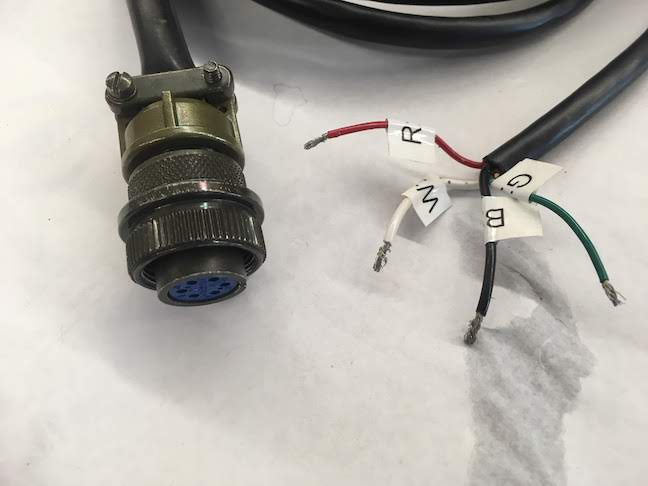
\includegraphics[width=0.8\linewidth]{pictures/6-pin-cable} 

}

\caption{6-pin cable to trigger a sampling sequence to the MUX, using the black (M-) and green (M+) wires, and, to communicate between the MUX and the spectro::lyser using the white (A+) and the red (B-) wires through the RS485 protocol}\label{fig:6-pin-cable}
\end{figure}

As illustrated in Figure \ref{fig:ConnectBox1}, insert the green ``M+'' wire at the bottom or left connection, and the black ``M-'' wire at the top or right connection of the `Valve' terminal.

\hypertarget{communications-between-the-mux-and-the-spectrolyser}{%
\subsection{Communications between the MUX and the Spectro::lyser}\label{communications-between-the-mux-and-the-spectrolyser}}

With this version, the MUX essentially takes control of the Spectro::lyser, by giving impoing the measurement intervals, the 12V trigger signal duration, and its time before measurements, sending it into `logger mode', and writing the fingerprint values onto an SD card. For this we use the RS485 protocol and connections available through the Con::nect Box.

As illustrated in Figure \ref{fig:ConnectBox1}, insert the white ``A+'' wire at the bottom or left connection, and the red ``B-'' wire at the top or right connection of the `RS485' terminal.

\hypertarget{the-mux-external-plugs}{%
\subsection{The MUX external plugs}\label{the-mux-external-plugs}}

The 6-pin and 2-pin wires are plugged in the MUX box itself via the ``Auxilliary'' and ``12 VDC'' plugs located on the hinge side of the MUX box as illustrated in Figure \ref{fig:ConnectBox1} below.

\begin{figure}

{\centering 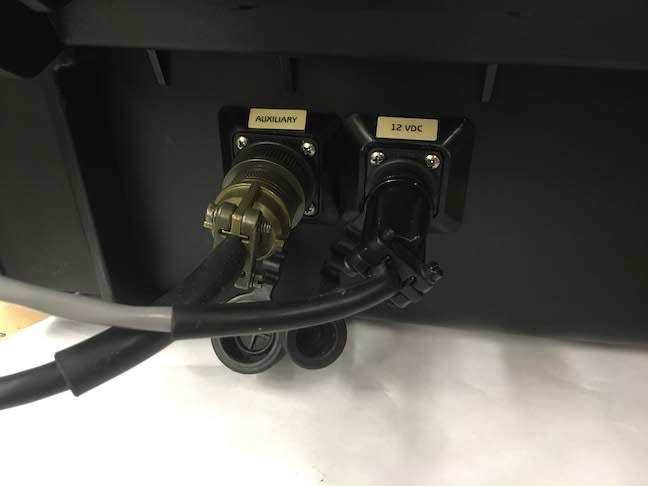
\includegraphics[width=0.8\linewidth]{pictures/ExternalPlugs} 

}

\caption{External plugs for the 2-pin and 6-pn cables}\label{fig:ExternalPlugs}
\end{figure}

\hypertarget{control-box-plugs}{%
\subsection{Control box plugs}\label{control-box-plugs}}

Inside the MUX, the control box (Figure \ref{fig:MUXLayout}) itself is connected via plugs to the 2-pin and 6-pin wires, and to the solenoid valves. The peristaltic pump is directly connected via its wires thanks to a screw terminal. Normally, there is no need to ever touch at any of these plugs. But should the user need it, it is possible to undo the control box from the rest, and or to change a solenoid valve and easily replace it if needed.

For illustration, the MUX power plugs, as well as the valve and the RS485 plugs on the control box. The 12V coming from the Con::nect Box are plugged in the control box as illustrated in Figure \ref{fig:ControlBoxConnection12V} below.

\begin{figure}

{\centering 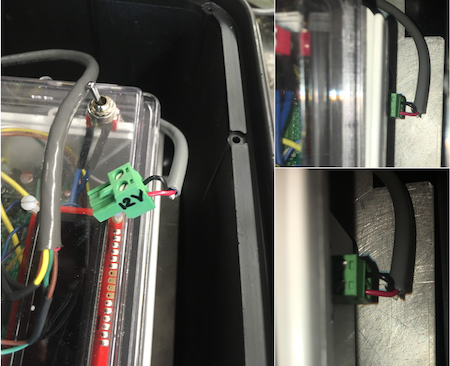
\includegraphics[width=0.8\linewidth]{pictures/ControlBoxConnection12V} 

}

\caption{12 V Connection between the control box and the external plug}\label{fig:ControlBoxConnection12V}
\end{figure}

The Signal input and the communication wires coming from the Con::nect Box are plugged in the control box as illustrated in Figure \ref{fig:ControlBoxConnectionValveRS485} below.

\begin{figure}

{\centering 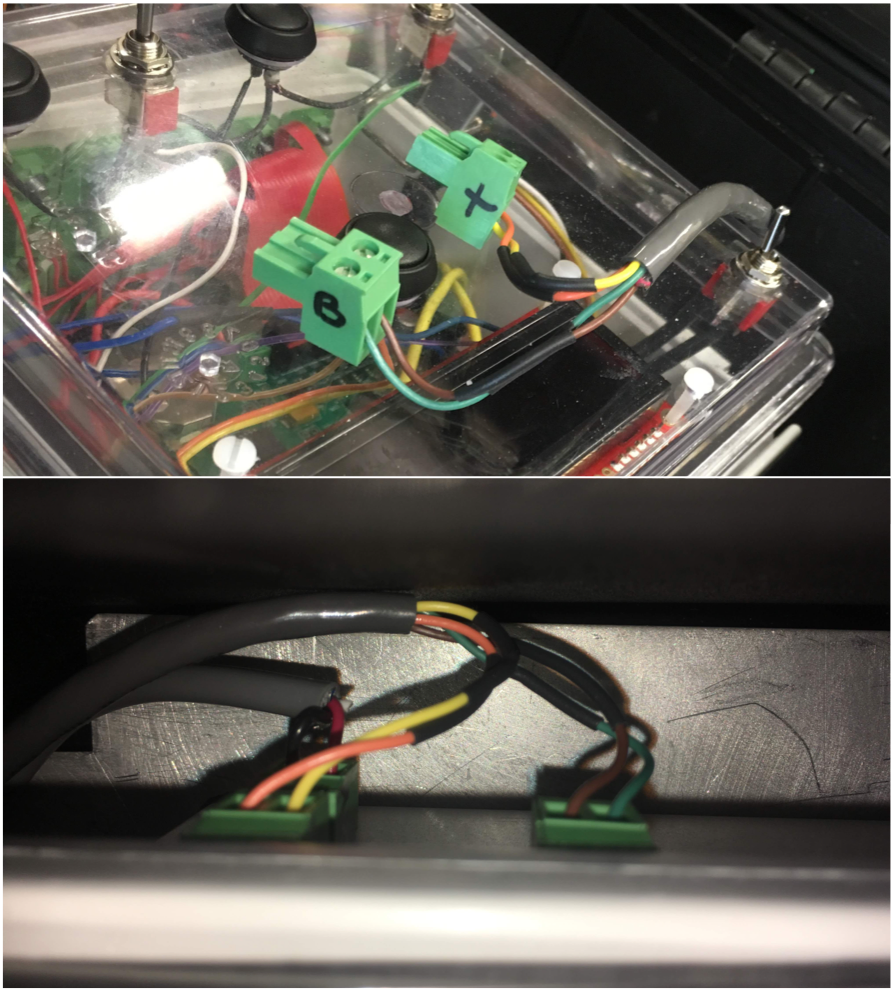
\includegraphics[width=0.8\linewidth]{pictures/ControlBoxConnectionValveRS485} 

}

\caption{12 V Connection between the control box and the external plug}\label{fig:ControlBoxConnectionValveRS485}
\end{figure}

\hypertarget{the-mux-sensor-functioning}{%
\chapter{The MUX-sensor functioning}\label{the-mux-sensor-functioning}}

\hypertarget{the-general-design-principles-for-the-mux}{%
\section{The general design principles for the MUX}\label{the-general-design-principles-for-the-mux}}

An exert from our first paper \citep{Birgand2016-to} summarizes the philosophy behind the MUX:

\begin{quote}
To remain affordable, the system uses a single high frequency automatic water quality probe as the central analytical
instrument to which water from different sampling sites (hereafter, point sources) are pumped via {[}the MUX{]}. Our design criteria when constructing the {[}MUX{]} system were: (1) to have the capacity of obtaining hourly or sub-hourly samples for measuring multiple point sources, (2) to be able to pump water from the point sources to the probe to overcome at least 3 m of head difference, (3) to be able to run on 12 volts (V) direct current (DC) power for field deployment, and (4) that the coupled {[}MUX{]}-water quality probe system functioned entirely automatically. An acceptable compromise for these criteria was to design {[}the MUX{]} that enabled sampling from up to 12 point source sites located within {[}30{]} m of the central probe. {[}\ldots{}{]}.
\end{quote}

\begin{quote}
As the in situ field spectrophotometer can only collect one measurement at a time on fixed time intervals, we designed and built {[}the MUX{]} to sequentially pump and purge water from each point source to the probe, in synchrony with the probe measurements, and cycle through the sequence of measurements to obtain at least hourly time resolution of data collection at each source. To maintain the water quality probe's capability of measuring small suspended particle concentrations, we chose 3.18 mm internal diameter flexible tubing as a sampling conduit of water from the point source to the probe, fitted with 1.5 mm mesh screens at the source {[}\ldots{}{]}. Consequently, the coupled {[}MUX{]}-water quality probe system is well suited for applications where the source sampling volume is not limited and does not affect the process or system studied.
\end{quote}

\hypertarget{the-different-parts-of-the-mux-sensor-system}{%
\section{The different parts of the MUX-sensor system}\label{the-different-parts-of-the-mux-sensor-system}}

\hypertarget{sampling-ports-and-rinsing-solutions}{%
\subsection{Sampling ports and rinsing solutions}\label{sampling-ports-and-rinsing-solutions}}

In continuous flow laboratory analytical equipment, the flow in the tubing is unidirectional, and the measuring cuvette is rinsed by the carrier solution and color reagent between samples to essentially eliminate cross-contamination between samples. In our case, although we are using the Spectro::lyser as an \emph{in situ} laboratory instrument, there is no carrier fluid for rinsing between samples. To minimize cross contamination between samples, the idea we developed was to reverse flow and purge the instrument cuvette from its water instead. This is the reason for using a peristaltic pump. Now water can be purged either to the sampling port or to a port dedicated to waste.

This addresses the cross contamination, but not the fouling that may occur as is often the case on the instrument optics. For this reason, the MUX has an embedded rinsing procedure where it is possible to use acid or other solutions for rinsing. The overall general MUX-sensor setup is summarized in Figure \ref{fig:WorkLayout} below.

\begin{figure}

{\centering 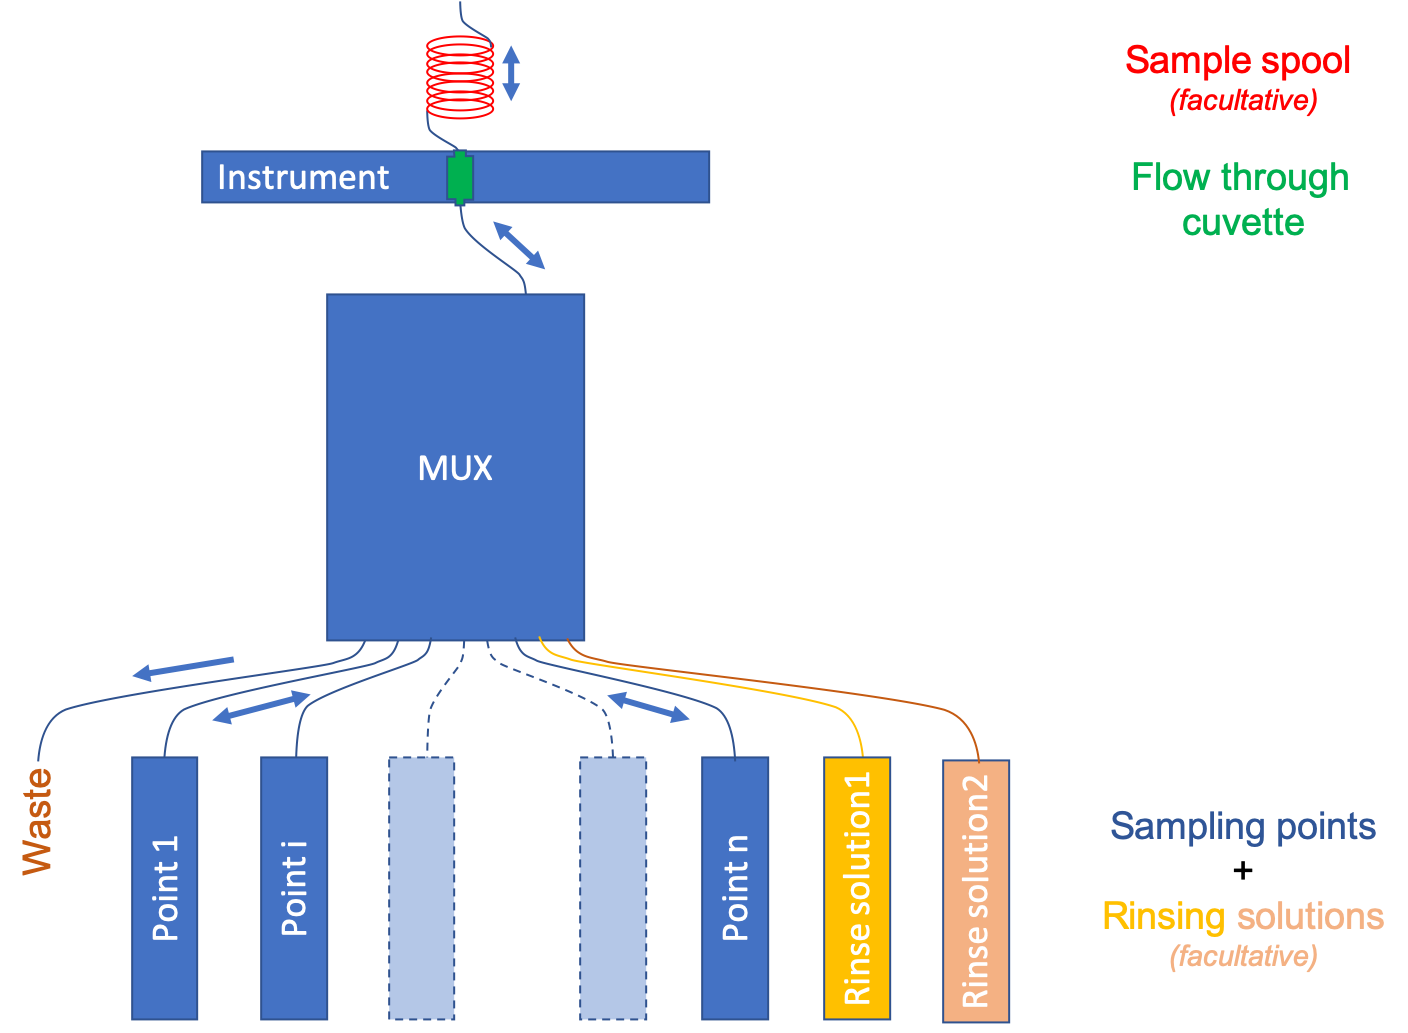
\includegraphics[width=0.8\linewidth]{pictures/WorkLayout} 

}

\caption{The MUX in relationship with the sampling points, rinsing solutions, the instrument and its flow-through cuvette, and a sample loop}\label{fig:WorkLayout}
\end{figure}

In Figure \ref{fig:WorkLayout} above, \emph{n} sampling ports are activated, while two of the ports are dedicated to a \emph{rinsing solution 1} and a \emph{rinsing solution 2}. The MUX has 12 sampling ports and a 13\textsuperscript{th} port for waste if desired. The number or rinsing solutions used, therefore reduces the number of available ports for measured points. In the case of Figure \ref{fig:WorkLayout} above, a maximum of 12 - 2 = 10 ports remain available for point sampling.

Sampled water from any sampling point, including the rinsing solutions, can be purged to any port, including the dedicated waste port (port 13 in the MUX box), or the same port used for sampling, or any other port of the user's choice.

\hypertarget{flow-through-cuvette}{%
\subsection{Flow through cuvette}\label{flow-through-cuvette}}

At the instrument, water is pumped through a flow-through cuvette. This allows to pump water beyond the cuvette and allow for rinsing of the whole manifold and of the cuvette with the new sample. We have found that a good practice to minimize cross contamination is to pump water at least 4 times beyond the volume of the cuvette. For use with the Spectro::lyser with a 35 mm opening, we recommend to use the cuvette 1-Q-10/SBTX2-8/10X20 from Starnacell\textsuperscript{®}. It has a 10 mm path length, is made of quartz, which lets the UV light through, and has a large collar, which make cleaning much easier.

\hypertarget{post-cuvette-sample-spool}{%
\subsection{Post-cuvette sample spool}\label{post-cuvette-sample-spool}}

Eventually during a measurement campaign, it is necessary to compare the instrument measured concentrations to those of the laboratory. For this, it is sometimes a good idea to add a \emph{sampling spool} made of tubing curled together. We recommend that the spool allows for large enough a volume corresponding to the one needed for lab analyses, but small enough such that the initial water that has served to rinse the MUX and the cuvette be beyond the spool such that when purging only `clean water' be used for lab sampling.

\hypertarget{sampling-sequences}{%
\section{Sampling sequences}\label{sampling-sequences}}

In the MUX \emph{config.txt} file (see further details later), the user specifies the desired sampling interval. During initialization, the MUX puts the Spectro::lyser in \emph{logger mode}, which means that the instrument will, with no live connection to a computer, automatically take measurements at the indicated time interval.

The Spectro::lyser sequence of actions (Figure \ref{fig:BasicSequence}) is thus to first send a 12V signal measurable at the `valve' output in the Con::nect box. Again, this is the way the Spectro::lyser deals with fouling. After a given time, referred to as \emph{clean wait} in the \emph{config.txt} file and in Figure \ref{fig:WorkLayout}, the instrument takes a measurement. A measurement consists in two series of light bursts accompanied by a series of beeps. There are about 9 seconds between the first and the last beep. After that, it takes the Spectro::lyser about 25 seconds to analyze its measurement and make available its absorbance fingerprint and its calculated concentrations (Figure \ref{fig:BasicSequence}).

\begin{figure}

{\centering 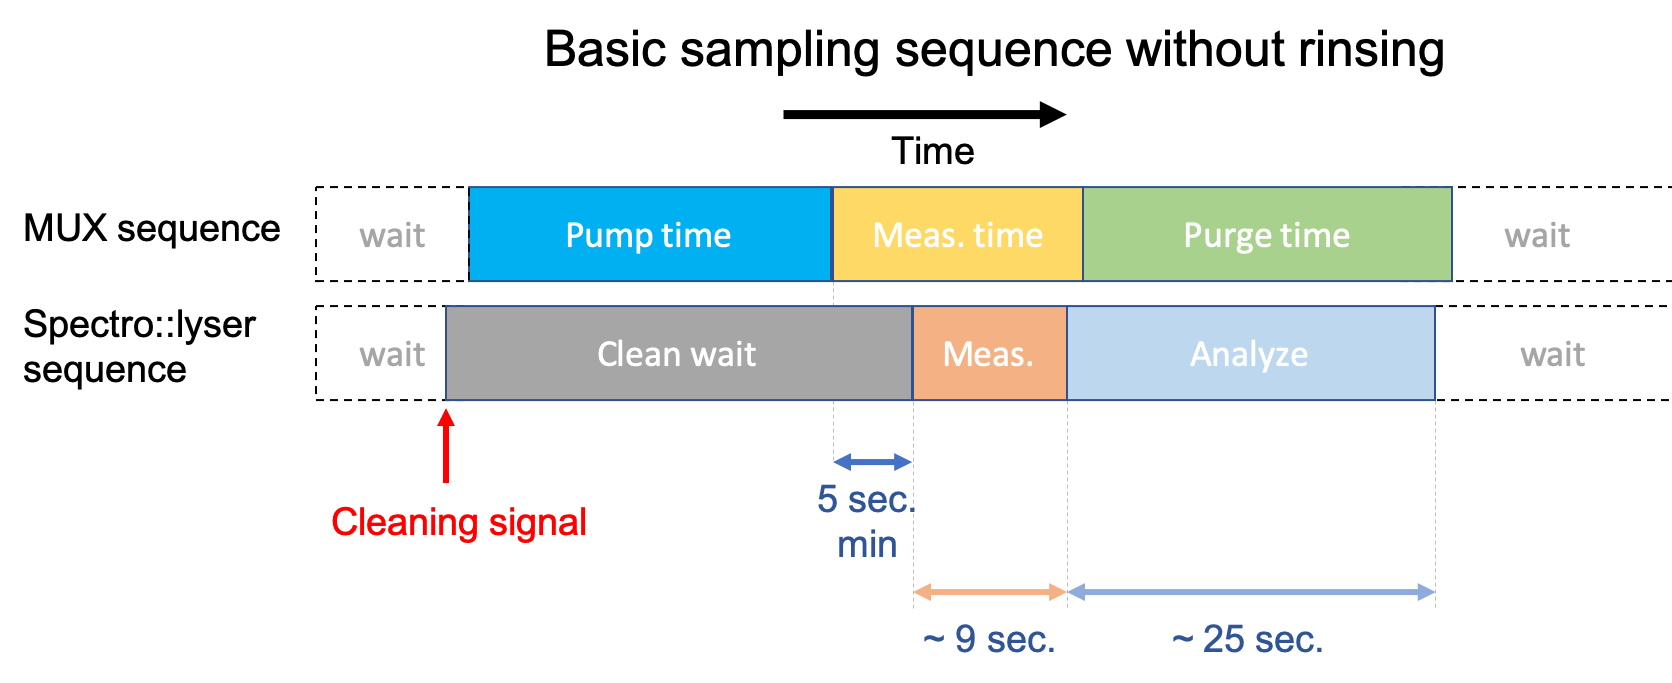
\includegraphics[width=0.8\linewidth]{pictures/BasicSequence} 

}

\caption{The MUX in relationship with the sampling points, rinsing solutions, the instrument and its flow-through cuvette, and a sample loop}\label{fig:BasicSequence}
\end{figure}

\hypertarget{pump-and-measurement-times}{%
\subsection{Pump and measurement times}\label{pump-and-measurement-times}}

The idea with the MUX is to have water to be analyzed in the measuring chamber or cuvette when the Spectro::lyser does its measurement. Once the MUX `hears' the \emph{cleaning signal} from the Spectro::lyser (Figure \ref{fig:BasicSequence}), it starts what we refer to as its \emph{sampling sequence}. The basic \emph{sampling sequence} consists in pumping, waiting for the Spectro::lyser measurement, and purging the MUX.

The MUX starts pumping for a \emph{pump time} defined in the \emph{config.txt} file for each valve or sampling port. The \emph{pump time} corresponds to the time it takes for water to go from its sampling point to the instrument cuvette, to which one must add the number of seconds necessary to rinse the equivalent of at least 4-5 times the cuvette volume \citep{Birgand2016-to}. For some applications, there is no limit on the available volume of water to be analyzed. In these cases, one might want to add 5-6 seconds more on the \emph{pump time}. For other applications, the available volume might be limited, and it might be necessary to limit the pump time to the strict minimum prescribed here.

The \emph{pump time} and the \emph{clean wait} times are thus intrinsically linked. The \emph{clean wait} time has to be equal to the pump time plus at least 5 seconds to let water in the cuvette `rest' and let all micro air bubbles to stop moving to obtain a reliable and consistent reading by the Spectro::lyser. Keep in mind that there are about 1-2 seconds delay between the \emph{cleaning signal} and the time when the pumping starts (Figure \ref{fig:BasicSequence}).

There are two important additional things to realize here:

\begin{enumerate}
\def\labelenumi{\arabic{enumi}.}
\item
  In reality, the \emph{pump time} may vary from sampling point to the next as it is preferable to pump the least amount of time per port to save energy and pump tubing. The \emph{pump time} for each port is defined in the \emph{config.txt} file. However, the \emph{clean wait} time corresponds to a parameter from the Spectro::lyser, and the same value applies to all sampling points. As a result, the \emph{clean wait} time \textbf{must correspond to the longest \emph{pump time} + 5 seconds} (Figure \ref{fig:TimingsSeveralPorts}).
\item
  Because it always takes the same amount of time between the \emph{cleaning signal} and the last beep of the Spectro::lyser measurement, and, because the \emph{pump time} may vary from one sampling point to the next, the (on the MUX side) \textbf{sum of \emph{pump time} + the MUX \emph{measurement time}} should also be the same and be equal to (on the Spectro::lyser side) \textbf{the \emph{clean wait} time + the 9 sec.~of measurement time + at least 2 seconds past the last measurement} (Figure \ref{fig:TimingsSeveralPorts}).
\end{enumerate}

As a result, the \emph{pumping time} and the \emph{measurement time} from the MUX must be adjusted (in the \emph{config.txt} file) accordingly for each sampling point as illustrated in Figure \ref{fig:TimingsSeveralPorts}

\begin{figure}

{\centering 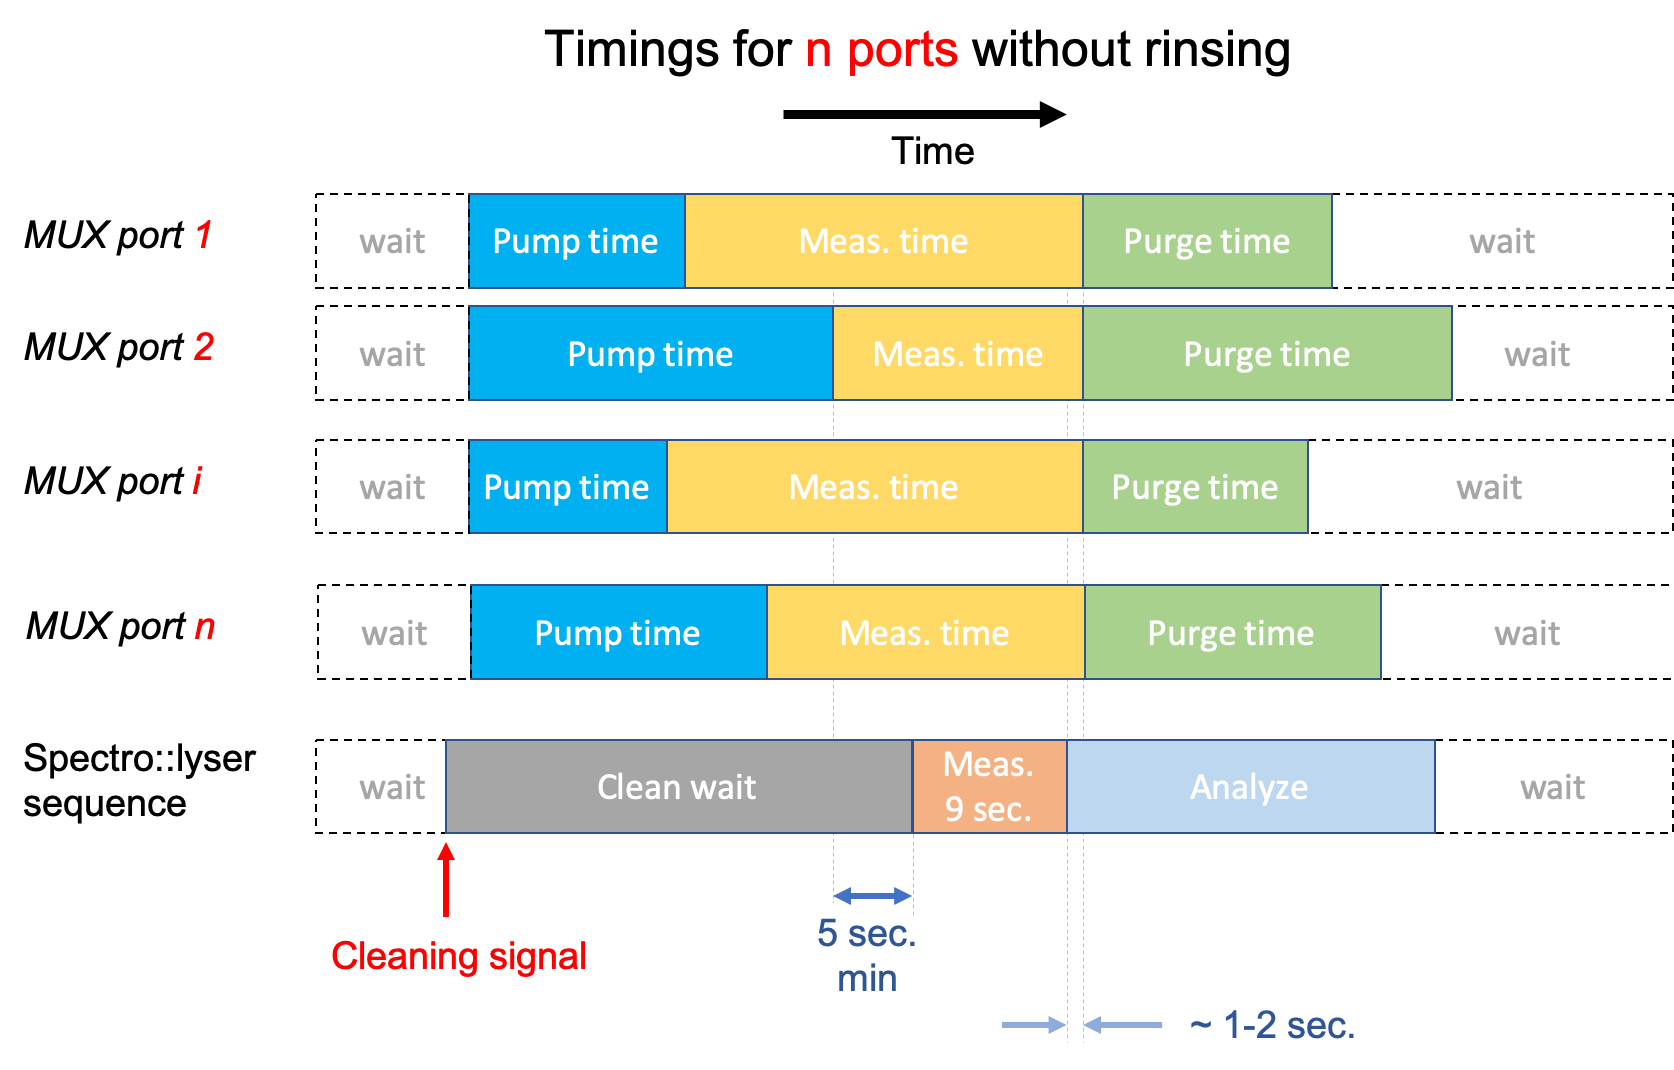
\includegraphics[width=0.8\linewidth]{pictures/TimingsSeveralPorts} 

}

\caption{Adjusting the *pumping times* and *measurement times* of the MUX to match the sequence of events of the Spectro::lyser}\label{fig:TimingsSeveralPorts}
\end{figure}

\hypertarget{purge-port-and-times}{%
\subsection{Purge port and times}\label{purge-port-and-times}}

The MUX \emph{purge time} corresponds to the time needed to purge, at least, the cuvette and the MUX valve manifold (Figure \ref{fig:MUXLayout}). The purge valve and the \emph{purge time} is defined in the \emph{config.txt} file. Depending on the application, the user might want:

\begin{itemize}
\tightlist
\item
  to purge the line that was just used for sampling all the way, in which case, we recommend to use the \emph{pump time} and add 3-4 seconds to make sure the line is rid of as many droplets as possible.
\item
  to purge to a \emph{waste} port (port 13 is the dedicated port for that but any port or valve can be used). In that case, the \emph{purge time} may be much shorter as in all likelihood the line to waste will be much shorter. The idea here is to save energy and the lifetime of the peristaltic pump tubing.
\end{itemize}

\hypertarget{sampling-sequence-with-automatic-rinsing}{%
\subsection{Sampling sequence with automatic rinsing}\label{sampling-sequence-with-automatic-rinsing}}

Our experience with the Spectro::lyser has suggested that a rinsing system be put in place to keep optics or cuvette fouling at a minimum. For this we have designed an embedded automatic \emph{rinsing sequence} that takes place right after the purging of the \emph{basic sampling sequence}. For this it is possible in the \emph{config.txt} file to define one or several \emph{rinsing sequence}. For each \emph{rinsing sequence}, one defines in the \emph{config.txt} file, the port from which the rinsing solution will be sampled and will be purged, the \emph{pumping time}, and the \emph{purging time} for the defined rinsing sampling and purging ports, and the number of seconds the rinsing solution will stay in the cuvette.

We have found that when water is sampled from areas where reduced conditions prevail, chemical fouling in the form of iron and manganese precipitate may occur. In these cases, we have found that rinsing using 5\% HCl acid solution or an oxalic acid solution (\textasciitilde{}15 mg L\textsuperscript{-1}) left in the cuvette for 1 min greatly reduced the amount of fouling. We have also found that in some cases rinsing with DI water is enough. In this case, the amount of time DI water stays in the cuvette does not matter as much and can be just a few seconds. We recommend that a \emph{rinsing sequence} that uses acid should be followed by a second rinsing sequence that uses DI water.

The timings for the \emph{rinsing sequence} are defined in the \emph{config.txt} file and the number of \emph{rinsing sequences} are also defined in the same file. The \emph{rinsing sequence(s)} automatically take(s) place after the \emph{purging} of the \emph{basic sampling sequence}, and does not require a \emph{cleaning signal} from the Spectro::lyser to take place as illustrated in Figure \ref{fig:BasicSequenceWith1Rinsing} below.

\begin{figure}

{\centering 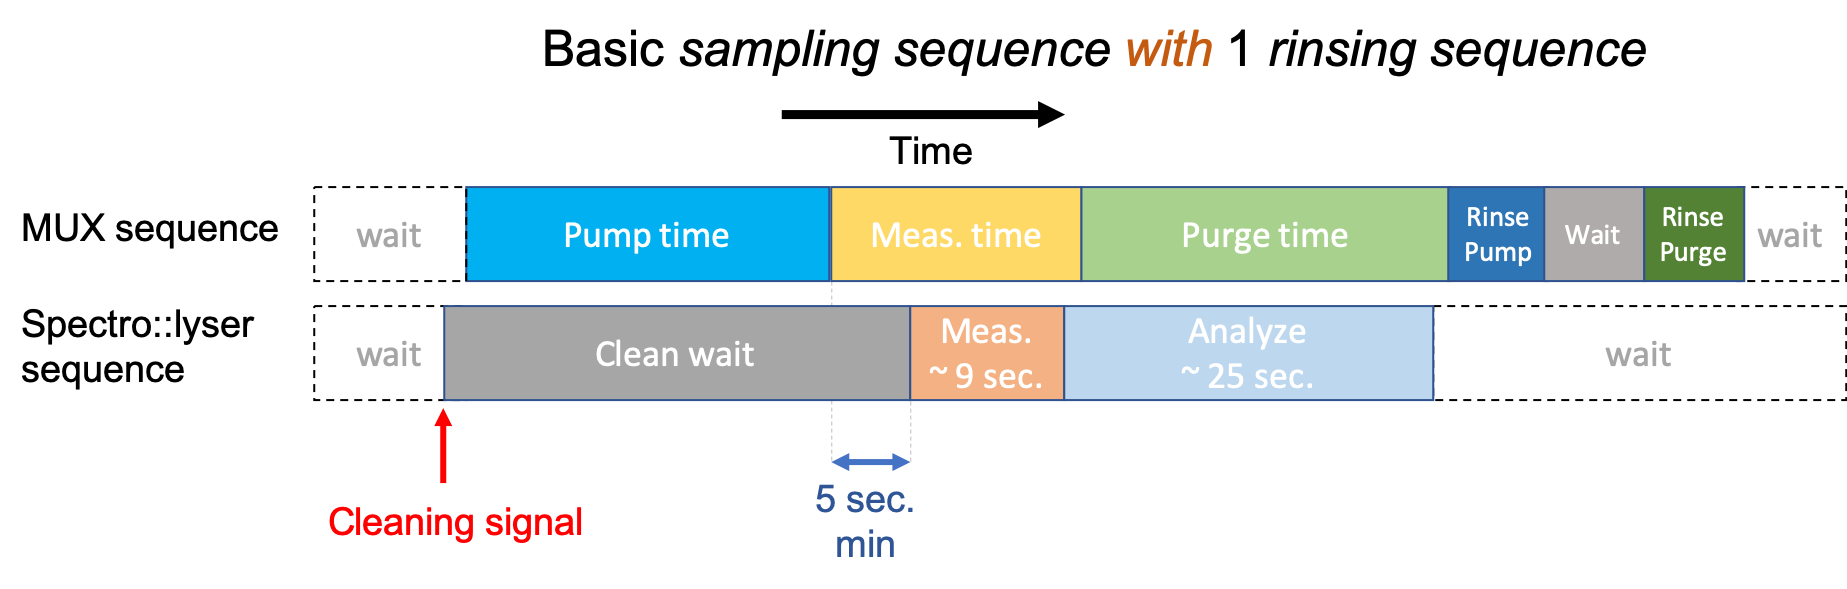
\includegraphics[width=1\linewidth]{pictures/BasicSequenceWith1Rinsing} 

}

\caption{The MUX *basic sampling sequence* followed by an automatic *rinsing sequence*}\label{fig:BasicSequenceWith1Rinsing}
\end{figure}

\hypertarget{sampling-cycle}{%
\section{Sampling cycle}\label{sampling-cycle}}

A \emph{sampling cycle} is the name we have given for a series of \emph{sampling sequences} that occur on a recurrent basis. For example, if the user has ports 1, 2, 4, and 5 being sampled, a \emph{sampling cycle} will have a \emph{sampling sequence} corresponding to port 1, followed by a \emph{sampling sequence} corresponding to port 2, etc., until the last sampled port, in our example, a \emph{sampling sequence} for port 5. This would make for the basic \emph{sampling cycle}. However, we do recommend that the user adds in the \emph{sampling cycle}, either air or DI water as an easily recognizable `tracer' measurement in the time series of fingerprint from the Spectro::lyser. In our example, a \emph{sampling cycle} would thus be: ``port 1, port 2, port 4, port 5, air'' or ``port 1, port 2, port 4, port 5, DI''. This \emph{sampling cycle} repeats itself indefinitely (Figure \ref{fig:SamplingCycle}). The example below only considers 4 sampled points, because there was not enough space for illustration. However, with one rinsing solution, and using air as a measurement tracer, a \emph{sampling cycle} can have up to 11 sampled ports (12 minus the port used for rinsing). With two rinsing solutions, and using air as a measurement tracer, a \emph{sampling cycle} would have up to 10 sampled ports (12 minus the 2 ports used for rinsing). In the latter case, one of the rinsing solutions would likely be DI water, which could also be used as the measurement tracer instead or air in the \emph{sampling cycle}. In that case, a \emph{sampling cycle} would still have up to 10 sampled ports (12 minus the 2 port used for rinsing, knowing that DI is used both for rinsingn and as a measurement tracer).

\begin{figure}

{\centering 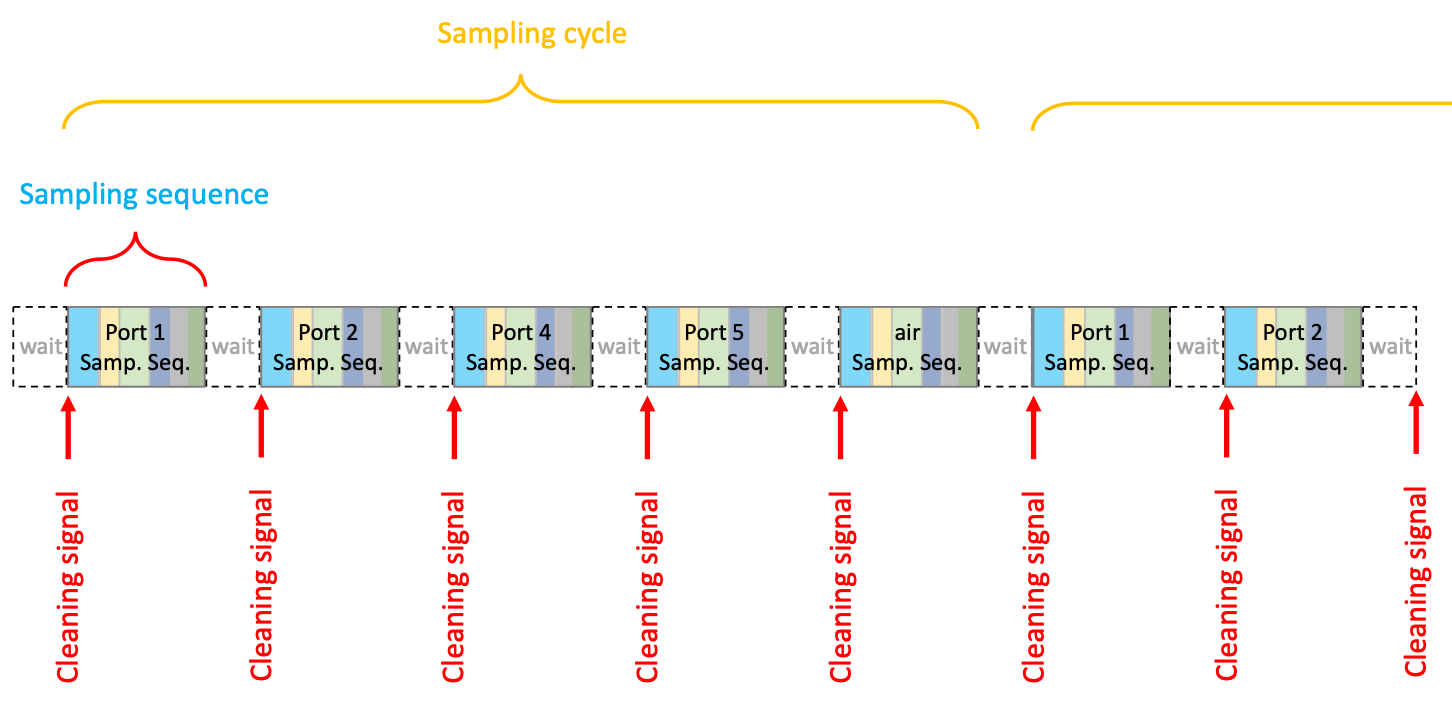
\includegraphics[width=1\linewidth]{pictures/SamplingCycle} 

}

\caption{The MUX *sampling sequences* for ports 1, 2, 4, and 5, included into *sampling cycles* in which an *air* measurement has been inserted}\label{fig:SamplingCycle}
\end{figure}

The advantage of inserting air or DI water in the \emph{sampling cycle} is that in addition to the aid it provides to identify each cycle in the fingerprint time series, it also gives an estimate of the fouling of the cuvette or the optics. To insert and \emph{air} measurement in the \emph{sampling cycle}, the user can use `port 13' in the \emph{config.txt} file as it is used for waste and is therefore open to the atmosphere. To insert an \emph{DI} measurement, the user has to have a dedicated port sampling DI from an container with enough DI volume to cover the field visit intervals.

\hypertarget{programing-the-mux}{%
\chapter{Programing the MUX}\label{programing-the-mux}}

\hypertarget{the-sd-card-in-the-control-box}{%
\section{The SD card in the control box}\label{the-sd-card-in-the-control-box}}

All the instructions for programing the MUX are consigned in the \emph{config.txt} file, itself located on the micro SD card. The SD card can be retrieved by opening the control box. One may use the macro SD card adapter provided to read the SD card on a computer (Figure \ref{fig:ControlBoxSDCard}).

\begin{figure}

{\centering 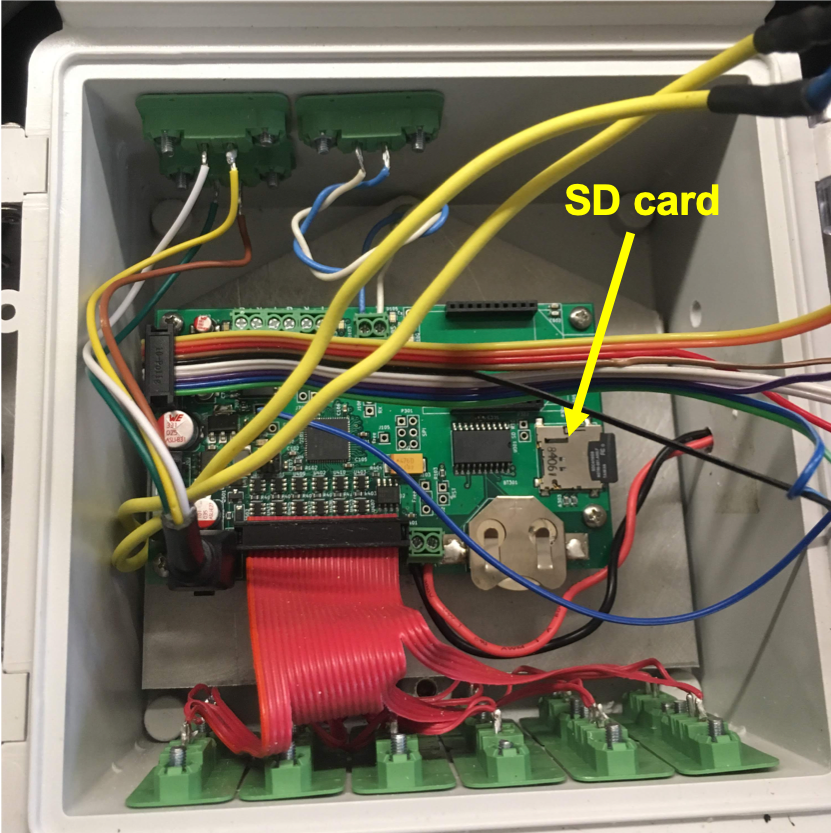
\includegraphics[width=0.7\linewidth]{pictures/ControlBoxSDCard} 

}

\caption{Location of the SD card in the control box of the MUX}\label{fig:ControlBoxSDCard}
\end{figure}

\hypertarget{the-config.txt-file}{%
\section{\texorpdfstring{The \emph{config.txt} file}{The config.txt file}}\label{the-config.txt-file}}

All the instructions for the sampling sequences are provided in the \emph{config.txt}. A typical basic \emph{config.txt} file looks like in Figure \ref{fig:ConfigBasic} below. In this particular example, there are 12 valves activated in a \emph{sampling cycle} ranked in increasing order from 1 to 12. The order of the valves can be completely interchanged and the \emph{sampling cycle} will go followin the prescribed order.

\begin{figure}

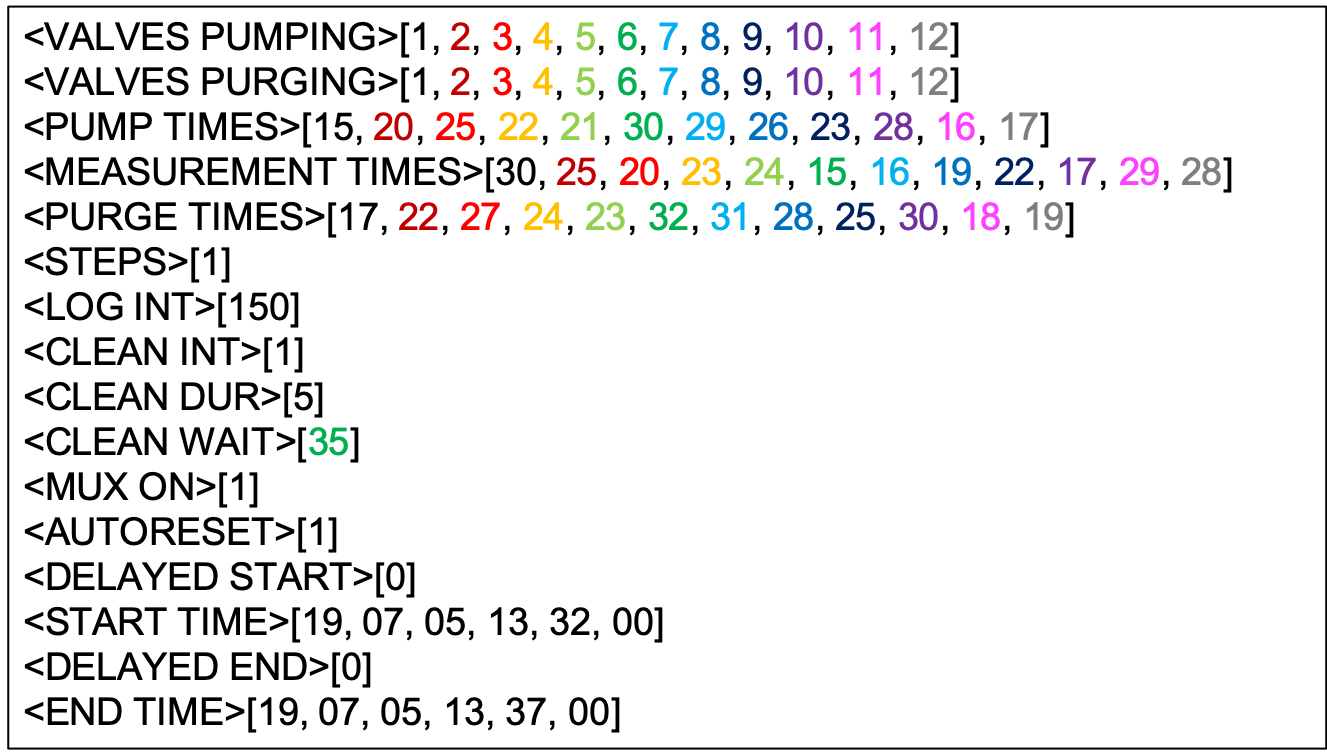
\includegraphics[width=0.6\linewidth]{pictures/ConfigBasic} \hfill{}

\caption{Typical *config.txt* file where 12 ports are activated, with no automatic rinsing}\label{fig:ConfigBasic}
\end{figure}

\hypertarget{programming-the-mux-sampling-sequence-without-automatic-rinsing}{%
\subsection{\texorpdfstring{Programming the MUX \emph{sampling sequence} without automatic rinsing}{Programming the MUX sampling sequence without automatic rinsing}}\label{programming-the-mux-sampling-sequence-without-automatic-rinsing}}

The commands for the \emph{sampling sequences} for each \emph{sampling cycle} are given in the first 6 lines of the \emph{config.txt} file (Figure \ref{fig:ConfigBasicMUXPart}). Each variable between \texttt{\textless{}...\textgreater{}} defines the name of the variable used in the program, and all numbers between \texttt{{[}...{]}} define the array of values to be used. The values in one array correspond to all the values necessary for a \emph{sampling cycle}.

\begin{figure}


\includegraphics[width=0.6\linewidth]{pictures/ConfigBasicMUXPart} \hfill{}

\caption{The commands for the MUX sampling sequence timing are provided in the first 6 lines of the *config.txt* (12 ports are activated, with no automatic rinsing)}\label{fig:ConfigBasicMUXPart}
\end{figure}

\begin{itemize}
\tightlist
\item
  \texttt{\textless{}VALVES\ PUMPING\textgreater{}} defines the list and its order of the valves or port which will be activated during \emph{pumping} of the \emph{sampling cycles}. In the example of Figure \ref{fig:ConfigBasicMUXPart}, the \emph{sampling cycles} inclues all valves from 1 to 12 in that order.
\item
  \texttt{\textless{}VALVES\ PURGING\textgreater{}} defines the list and its order of the valves or port which will be activated during the \emph{purging} phase of each \emph{sampling sequence} of the \emph{sampling cycle}. In the particular example of Figure \ref{fig:ConfigBasicMUXPart}, all water is purged back to \emph{its source} as the same valve is used during \emph{pumping} and \emph{purging}.
\item
  \texttt{\textless{}PUMP\ TIMES\textgreater{}} defines the array of values in seconds that will be used for the \emph{pumping} in each \emph{sampling sequence} corresponding to the \emph{pumping} valve activated.
\item
  \texttt{\textless{}MEASUREMENT\ TIMES\textgreater{}} defines the array of values in seconds that will be used for each \emph{sampling sequence} and corresponding to the activated valve.
\item
  \texttt{\textless{}PURGE\ TIMES\textgreater{}} defines the array of values in seconds that will be used for the \emph{purping} in each \emph{sampling sequence} corresponding to the \emph{purging} valve activated.
\item
  \texttt{\textless{}STEPS\textgreater{}{[}1{]}} means that there is no automatic rinsing. Technically, it defines the fact that the program will read each array and each cleaning signal will activate the next \texttt{{[}1{]}} (one) value in the array. In other words, the program will read the next value in the array to be used upon a \emph{cleaning signal} (more details later).
\end{itemize}

For illustration purposes, the text of the \emph{config.txt} file have been colored. In the current example (Figure \ref{fig:ConfigBasicMUXPart}), in the \emph{sampling cycle}, the first \emph{sampling sequence} starts with pumping from valve 1 for 15 seconds, waits for 30 sec for the Spectro::lyser to do its measurement, then purge to through the same valve 1 for 17 seconds, i.e., 2 seconds more than pumping to remove as many drops as possible. Because the \texttt{\textless{}STEPS\textgreater{}} is set to 1, the MUX waits for the next Spectro::lyser \emph{cleaning signal} to start its next \emph{sampling sequence}.

By analogy, the 7\textsuperscript{th} \emph{sampling sequence} starts with pumping from valve 7 for 29 seconds, waits for 16 sec for the Spectro::lyser to do its measurement, then purge to through the same valve 7 for 31 seconds, i.e., 2 seconds more than pumping to remove as many drops as possible.

\begin{itemize}
\item
  Notice that for all activated valves, \texttt{\textless{}PUMP\ TIMES\textgreater{}\ +\ \textless{}MEASUREMENT\ TIMES\textgreater{}} is always equal to 45 seconds, and the 45 seconds corresponds to the longest \emph{pumping time} (30 sec, corresponding to valve 6 in the example), plus 5 seconds of no pumping for all gas bubbles to settle, plus 9 seconds for the Spectro::lyser measurement to take place. The current setting suggests that the MUX would start its purging not even one second after the last beep of the Spectro::lyser measurement\ldots{} That would work, but honestly there is advantage to do that. So adding several seconds more in the measurement timings would probably be more judicious and safer to make sure water is still in the cuvette for the full measurement.
\item
  Also notice that the \texttt{\textless{}PUMP\ TIMES\textgreater{}\ +\ \textless{}MEASUREMENT\ TIMES\textgreater{}} is equal to the \texttt{\textless{}CLEAN\ WAIT\textgreater{}} (Figure \ref{fig:ConfigBasic}) value minus 5 seconds corresponding to the minimum of time for bubbles to settle for the longest pumping time (more details below)
\end{itemize}

\hypertarget{programming-the-mux-sampling-sequence-with-two-automatic-rinsing-and-a-waste-port}{%
\subsection{\texorpdfstring{Programming the MUX \emph{sampling sequence} with two automatic rinsing, and a waste port}{Programming the MUX sampling sequence with two automatic rinsing, and a waste port}}\label{programming-the-mux-sampling-sequence-with-two-automatic-rinsing-and-a-waste-port}}

The next example illustrates more complicated options. The user wants to use points 10, 1, 3, 8, 9, 2 in that order in a \emph{sampling cycle} and wants to add an \emph{air tracer measurement}. The user does not want to purge water back to the sampling point, but rather, wants to purge all water to a waste port, which incidently can be used for lab sampling purposes. The user also wants to use two automatic rinsing, the first one with acid where acid would stay in the cuvette for 55 seconds to leave enough reaction time, and the second one with DI to rinse the acid off.

The MUX could be programed as illustrated in Figure \ref{fig:Config2rinsesMUXPart} below.

\begin{figure}

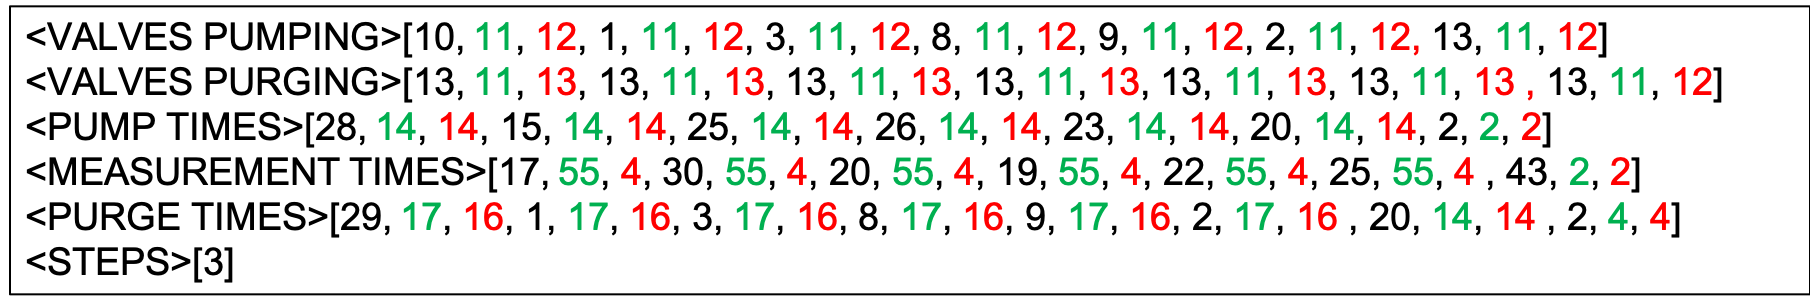
\includegraphics[width=0.8\linewidth]{pictures/Config2rinsesMUXPart} \hfill{}

\caption{Programing for 6 ports and an air measurement, purging to waste, and two automatic rinsing}\label{fig:Config2rinsesMUXPart}
\end{figure}

\begin{itemize}
\tightlist
\item
  Notice that \texttt{\textless{}STEPS\textgreater{}} value is set to 3. This means that the MUX \emph{sampling sequence} will be activated by the \emph{cleaning signal} every 3 values of the arrays (the text in black in Figure \ref{fig:Config2rinsesMUXPart}). In between, the green and red values, are automatically activated during the \emph{sampling sequence}, and correspond here to the two rinsing desired. The green values corresponds to the values for the acid rinse, and the red values correspond to the DI rinse.
\item
  The activated sampling ports (other than rinsing) of the \emph{sampling cycle} are defined in the \texttt{\textless{}VALVES\ PUMPING\textgreater{}} array and appear in black in Figure \ref{fig:Config2rinsesMUXPart}. Their list is thus 10, 1, 3, 8, 9, 2, and 13. The last one, 13, corresponds to the waste port open to the atmosphere, which means that it can be used for `air tracer measurement'.
\item
  The port used for purging of the sampled points (other than rinsing) also appears in black in the \texttt{\textless{}VALVES\ PURGING\textgreater{}}
  array, and is always 13.
\item
  The pump times, measurement times, and purge times for the sampled points are illustrated in black, respectively, in the \texttt{\textless{}PUMP\ TIMES\textgreater{}}, \texttt{\textless{}MEASUREMENT\ TIMES\textgreater{}}, and \texttt{\textless{}PURGE\ TIMES\textgreater{}} arrays (Figure \ref{fig:Config2rinsesMUXPart})
\item
  The acid rinse will be pumped and purged from and to port 11 everytime. There often no need to purge acid to waste. Although, the low strength of the acid would not damage the environment, it is preferable to purge back to its bottle to save acid. The dilution by water droplets will not affect acid strength and anti-fouling efficacy.
\item
  To leave acid in the cuvette for 55 seconds, the user add 55 sec.~in the \texttt{\textless{}MEASUREMENT\ TIMES\textgreater{}} array.
\item
  The DI water rinse is always pumps from port 12 in the example from a designated DI water jar. In the example, the DI water is purged to the waste port 13. This implies that a lrge enough DI water container be used to have enough between field service intervals.
\item
  The amount of time DI water stays in the cuvette does not matter as much as acid here and a value of 4 seconds has been chosen in the example.
\item
  During the air measurements, the pumping and purging times are kept to a minimum (2 sec.) to minimize energy spending and peristaltic pump wear. The measurement time (black value) is set to 43 seconds to stay in sequence with the other \emph{sampling sequences} although it could have been shortened as well.
\end{itemize}

\hypertarget{the-spectrolyser-values-in-the-config.txt-file}{%
\subsection{\texorpdfstring{The Spectro::lyser values in the \emph{config.txt} file}{The Spectro::lyser values in the config.txt file}}\label{the-spectrolyser-values-in-the-config.txt-file}}

The next five lines in the \emph{config.txt} file give instructions to the Spectro::lyser on the values to use when going into the \emph{logger mode} (Figure \ref{fig:ConfigScan}).

\begin{figure}

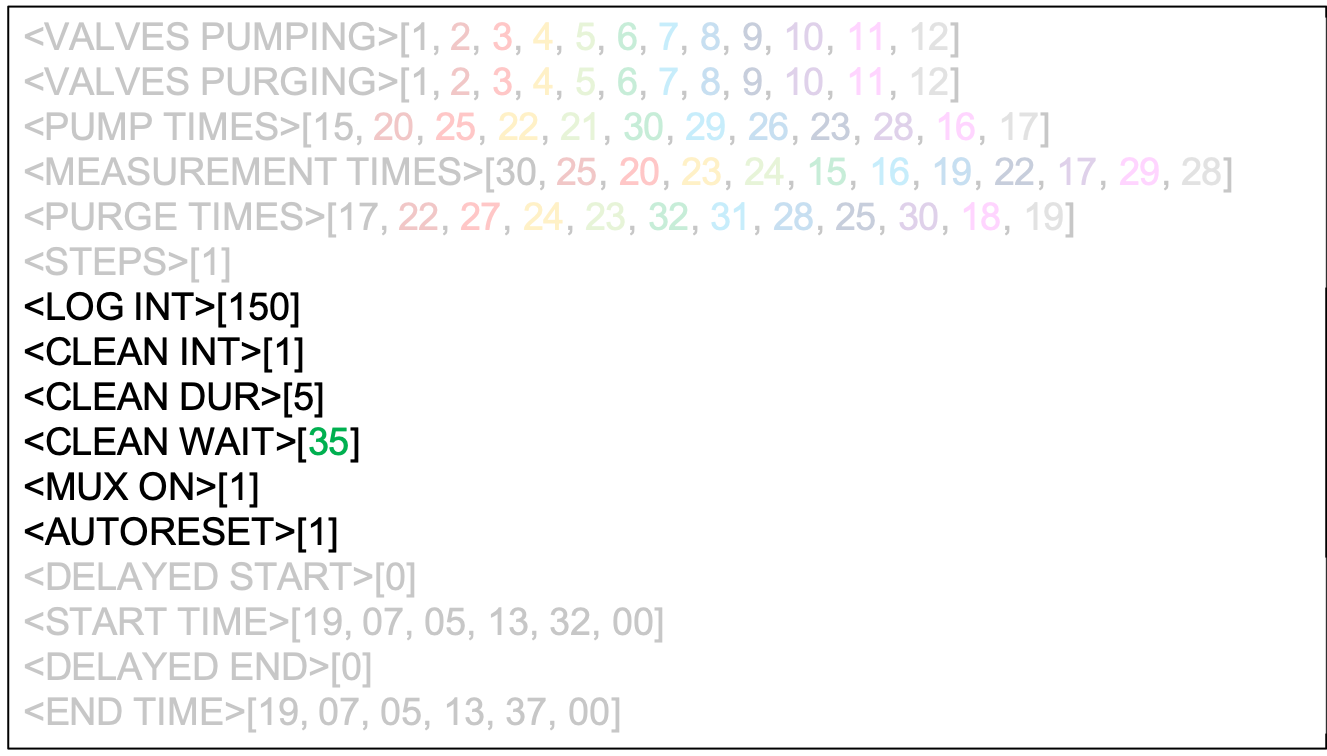
\includegraphics[width=0.6\linewidth]{pictures/ConfigScan} \hfill{}

\caption{The parameters in the *config.txt* to pilot the Spectro::lyser}\label{fig:ConfigScan}
\end{figure}

\begin{itemize}
\tightlist
\item
  \texttt{\textless{}LOG\ INT\textgreater{}} defines the interval in seconds, at which the Spectro::lyser will take a measurement and logs its value. It also corresponds to the interval at which the Spectro::lyser sends a \emph{cleaning signal}, which in the end corresponds at the time interval between two \emph{sampling sequences}. The time interval on each sampled point will be the recurring interval of a \emph{sampling cycle}.
\item
  \texttt{\textless{}CLEAN\ INT\textgreater{}} defines the number of \emph{logging intervals} or measurements from the Spectro::lyser there are before it sends a \emph{cleaning signal}. This does not apply to our use, as we want to have a \emph{cleaning signal} sent everytime the Spectro::lyser takes a measurement. ALWAYS set it to 1.
\item
  \texttt{\textless{}CLEAN\ DUR\textgreater{}} defines the number of seconds the 12V cleaning signal coming from the Spectro::lyser is on.
\item
  \texttt{\textless{}CLEAN\ WAIT\textgreater{}} defines the number of seconds between the beginning of the \emph{cleaning signal} and the first beep of the Spectro::lyser measurement. \textbf{The duration of this value is linked to the \emph{pumping times}, and must be equal, at least, to the \emph{longest} pumping time of the \emph{sampling cycle}, plus 5 seconds to leave time for air bubbles to settle}.
\item
  \texttt{\textless{}MUX\ ON\textgreater{}} has to be set at 1. It corresponds to a feature obsolete with the current version of MUX.
  \texttt{\textless{}AUTORESET\textgreater{}} this option defines whether the user wants the system to autorest at midnight everyday. We recommend to use this option (set to {[}1{]}), as it allows the MUX to clean up its memory. If the user prefers not to use this option, then set to {[}0{]}.
\end{itemize}

\hypertarget{delayed-start}{%
\subsection{Delayed start}\label{delayed-start}}

In many situations, it might be of advantage not to start sampling when the users are in the field, but rather start at a later time. Similarly, the user might want to stop the system before being able to come to the field to retrieve data. This what the delayed start and end are for. If the user does not want the delayed start and end, set \texttt{\textless{}DELAYED\ START\textgreater{}} and \texttt{\textless{}DELAYED\ END\textgreater{}} to {[}0{]}.

When the user wants a delayed start, set \textbf{both} \texttt{\textless{}DELAYED\ START\textgreater{}} and \texttt{\textless{}DELAYED\ END\textgreater{}} to {[}1{]}. The start time is defined in \texttt{\textless{}START\ TIME\textgreater{}} as {[}YY,MM,DD,HH,mm,SS{]}. When the user does not want the system to end until the next field visit, set the \texttt{\textless{}END\ TIME\textgreater{}} to several years later. An example is given below in Figure \ref{fig:ConfigDelay}.

\begin{figure}


\includegraphics[width=0.5\linewidth]{pictures/ConfigDelay} \hfill{}

\caption{Example of delayed start on the *config.txt* file}\label{fig:ConfigDelay}
\end{figure}

\hypertarget{examples-of-config.txt-files}{%
\section{\texorpdfstring{Examples of \emph{config.txt} files}{Examples of config.txt files}}\label{examples-of-config.txt-files}}

\textbf{Always make sure that there is the arrays in the \texttt{\textless{}VALVES\ PUMPING\textgreater{}}, \texttt{\textless{}VALVES\ PURGING\textgreater{}}, \texttt{\textless{}PUMP\ TIMES\textgreater{}}, \texttt{\textless{}MEASUREMENT\ TIMES\textgreater{}}, and \texttt{\textless{}PURGE\ TIMES\textgreater{}} all have the same number of values!!!}

\hypertarget{sampling-cycles-with-no-rinsing}{%
\subsection{Sampling cycles with no rinsing}\label{sampling-cycles-with-no-rinsing}}

\begin{itemize}
\tightlist
\item
  12 sampling ports in 1, 2, 3, 4, 5, 6, 7, 8, 9, 10, 11, 12 order.
\item
  same purging ports
\item
  Five minutes \emph{sampling sequence} intervals
\item
  60 time resolution for each sampled point
\end{itemize}

\begin{verbatim}
<VALVES PUMPING>[1, 2, 3, 4, 5, 6, 7, 8, 9, 10, 11, 12]
<VALVES PURGING>[1, 2, 3, 4, 5, 6, 7, 8, 9, 10, 11, 12]
<PUMP TIMES>[15, 20, 25, 22, 21, 30, 29, 26, 23, 28, 16, 17]
<MEASUREMENT TIMES>[30, 25, 20, 23, 24, 15, 16, 19, 22, 17, 29, 28]
<PURGE TIMES>[17, 22, 27, 24, 23, 32, 31, 28, 25, 30, 18, 19]
<STEPS>[1]
<LOG INT>[150]
<CLEAN INT>[1]
<CLEAN DUR>[5]
<CLEAN WAIT>[35]
<MUX ON>[1]
<AUTORESET>[1]
<DELAYED START>[0]
<START TIME>[19, 07, 05, 13, 32, 00]
<DELAYED END>[0]
<END TIME>[19, 07, 05, 13, 37, 00]
\end{verbatim}

\hypertarget{sampling-cycles-with-one-rinse}{%
\subsection{Sampling cycles with one rinse}\label{sampling-cycles-with-one-rinse}}

\begin{itemize}
\tightlist
\item
  4 sampling ports in 1, 3, 5, 7 order, no tracer measurement (not recommended)
\item
  one automatic (e.g., DI water) rinse on port 2
\item
  same purging ports
\item
  Three minutes \emph{sampling sequence} intervals
\item
  12 time resolution for each sampled point
\end{itemize}

\begin{verbatim}
<VALVES PUMPING>[1, 2, 3, 2, 5, 2, 7, 2]
<VALVES PURGING>[1, 2, 3, 2, 5, 2, 7, 2]
<PUMP TIMES>[10, 5,10, 5,10, 5,10, 5]
<MEASUREMENT TIMES>[12, 3, 12, 3, 12, 3, 12, 3]
<PURGE TIMES>[10, 3, 10, 3, 10, 3, 10, 3]
<STEPS>[2]
<LOG INT>[180]
<CLEAN INT>[1]
<CLEAN DUR>[5]
<CLEAN WAIT>[12]
<MUX ON>[1]
<AUTORESET>[1]
<DELAYED START>[0]
<START TIME>[19, 07, 06, 06, 08, 00]
<DELAYED END>[0]
<END TIME>[19, 07, 06, 13, 37, 00]
\end{verbatim}

\hypertarget{sampling-cycles-with-one-rinse-1}{%
\subsection{Sampling cycles with one rinse}\label{sampling-cycles-with-one-rinse-1}}

\begin{itemize}
\tightlist
\item
  4 sampling ports in 1, 3, 5, 7 order, one air tracer measurement (recommended)
\item
  one automatic (e.g., DI water) rinse on port 2
\item
  All purging on port 13
\item
  Three minutes \emph{sampling sequence} intervals
\item
  15 time resolution for each sampled point
\end{itemize}

\begin{verbatim}
<VALVES PUMPING>[1, 2, 3, 2, 5, 2, 7, 2, 13, 2]
<VALVES PURGING>[13, 2, 13, 2, 13, 2, 13, 2, 13, 2]
<PUMP TIMES>[10, 5,10, 5,10, 5,10, 5, 2, 2]
<MEASUREMENT TIMES>[12, 3, 12, 3, 12, 3, 12, 3, 2, 2]
<PURGE TIMES>[10, 3, 10, 3, 10, 3, 10, 3, 2, 2]
<STEPS>[2]
<LOG INT>[180]
<CLEAN INT>[1]
<CLEAN DUR>[5]
<CLEAN WAIT>[12]
<MUX ON>[1]
<AUTORESET>[1]
<DELAYED START>[0]
<START TIME>[19, 07, 06, 06, 08, 00]
<DELAYED END>[0]
<END TIME>[19, 07, 06, 13, 37, 00]
\end{verbatim}

\hypertarget{sampling-cycles-with-one-rinse-2}{%
\subsection{Sampling cycles with one rinse}\label{sampling-cycles-with-one-rinse-2}}

\begin{itemize}
\tightlist
\item
  4 sampling ports in 10, 1, 3, 8, 9, 2, and one air (13) tracer measurement (recommended)
\item
  two automatic, e.g., acid or port 11, followed by DI water rinse on port 12
\item
  All purging on port 13, but for acid back to port 11
\item
  Because of the two rinses, the interval between two \emph{sampling sequences} has to be a bit longer, in fact longer than the summation of the (pumping time + measurement time), the acid (pumping, stay in cuvette, purging) times, and the DI water (pumping, stay in cuvette, purging) times. That sum is equal to 164 seconds. So technically, one could set the log interval to 180 seconds. However, in practice, this would mean that the MUX would be pumping and purging a lot of the time, drawing lots of power and wearing out the peristaltic pump tubing. The user must also assess whether 30 min or hourly data is in fact plenty enough.
\item
  Five minutes \emph{sampling sequence} intervals
\item
  35 time resolution for each sampled point
\end{itemize}

\begin{verbatim}
<VALVES PUMPING>[10, 11, 12, 1, 11, 12, 3, 11, 12, 8, 11, 12, 9, 11, 12, 2, 11, 12, 13, 11, 12]
<VALVES PURGING>[13, 11, 13, 13, 11, 13, 13, 11, 13, 13, 11, 13, 13, 11, 13, 13, 11, 13 , 13, 11, 12]
<PUMP TIMES>[28, 14, 14, 15, 14, 14, 25, 14, 14, 26, 14, 14, 23, 14, 14, 20, 14, 14, 2, 2, 2]
<MEASUREMENT TIMES>[17, 55, 4, 30, 55, 4, 20, 55, 4, 19, 55, 4, 22, 55, 4, 25, 55, 4 , 43, 2, 2]
<PURGE TIMES>[29, 17, 16, 1, 17, 16, 3, 17, 16, 8, 17, 16, 9, 17, 16, 2, 17, 16 , 20, 14, 14 , 2, 4, 4]
<STEPS>[3]
<LOG INT>[300]
<CLEAN INT>[1]
<CLEAN DUR>[5]
<CLEAN WAIT>[33]
<MUX ON>[1]
<AUTORESET>[1]
<DELAYED START>[0]
<START TIME>[19, 07, 06, 06, 08, 00]
<DELAYED END>[0]
<END TIME>[19, 07, 06, 13, 37, 00]
\end{verbatim}

\hypertarget{the-files-saved-on-the-sd-card}{%
\chapter{The files saved on the SD card}\label{the-files-saved-on-the-sd-card}}

\hypertarget{the-mux-log-files}{%
\section{The MUX log files}\label{the-mux-log-files}}

All activities from the MUX are saved on a file named \emph{YYMM-MUX.txt}, with YY for the year, and MM for the month. A typical example of the content of the \emph{MUX.txt} file is illustrated below:

\begin{verbatim}
2019/7/4 10:32:36, 10, Forward, 10, 20, 5, Automatic - Start!
2019/7/4 10:33:06, 8, Reverse, 10, 20, 5, Automatic
2019/7/4 10:33:12, 2, Forward, 3, 15, 3, Automatic
2019/7/4 10:33:30, 2, Reverse, 3, 15, 3, Automatic
2019/7/4 10:35:35, 1, Forward, 15, 10, 8, Automatic
2019/7/4 10:36:00, 8, Reverse, 15, 10, 8, Automatic
2019/7/4 10:36:09, 2, Forward, 3, 20, 3, Automatic
2019/7/4 10:51:36, 10, Forward, 10, 20, 5, Automatic - Start!
2019/7/4 10:52:06, 8, Reverse, 10, 20, 5, Automatic
2019/7/4 10:52:12, 2, Forward, 3, 2, 3, Automatic
2019/7/4 10:52:17, 2, Reverse, 3, 2, 3, Automatic
2019/7/4 10:52:20, 7, Forward, 3, 2, 4, Automatic
2019/7/4 10:52:25, 3, Reverse, 3, 2, 4, Automatic
2019/7/4 10:53:36, 1, Forward, 15, 15, 8, Automatic
2019/7/4 10:54:06, 8, Reverse, 15, 15, 8, Automatic
2019/7/4 10:54:15, 2, Forward, 3, 2, 3, Automatic
2019/7/4 10:54:20, 2, Reverse, 3, 2, 3, Automatic
2019/7/4 10:54:23, 7, Forward, 3, 2, 4, Automatic
\end{verbatim}

On each line of the file, the first value is the time stamp of any pumping (\emph{Forward}) or purging (\emph{Reverse}) action. The next value is the valve or port that is activated. The next value is whether the pump pumped forward or purged for purging. The next three values correspond to . The next value tells whether the MUX actions were automatic, or whether the pumping and purging were done manually. When the MUX is started by turning the on/off button, or when the MUX is automatically reset at midnight, these actions are flagged by a `- Start!' at the end of the line.

This log file is very useful when trouble shooting and to corroborate information stored on the \emph{.fp} file.

\hypertarget{the-fingerprint-files}{%
\subsection{The fingerprint files}\label{the-fingerprint-files}}

The fingerprint files are a copy on the SD card of the fingerprint (.fp) stored by the Spectro::lyser. Until very recently, there was very limited memory space on the Spectro::lyser, leaving about three days of autonomy for 3-min measurements\ldots{} As a result, the MUX automatically interrogates the Spectro::lyser after each \emph{sampling sequence} and asks the Spectro::lyser to give the last absorbance spectrum stored in its memory, and appends it at the end of an \emph{.fp} file on the SD card.

An example of the such \emph{.fp} file is illustrated below. The first line defines which Spectro::lyser is used. The second line defines the Date/time, then status (OK or not), and then the wavelengths at which the absorbances are measured. In our case here, from 200.00 to 750.00 nm. The next lines provide the Spectro::lyser time stamp, the status of the probe, the absorbance values corresponding to each wavelength, AND, at the end of the line, the valve used for pumping and the time stamp from the MUX. The \texttt{...} replace all the 200 and some intermediate values on each line.

\begin{verbatim}
17240013_50_0x0101_spectro::lyser_RIV100NFV2
Date/Time   Status_0    200.00  202.50  ... 745.00  747.50  750.00
2019.07.04  10:51:59    Ok  42.7532 41.6454 ... nan nan nan 10  19/7/4 10:52
2019.07.04  10:51:59    Ok  42.7532 41.6454 ... nan nan nan 1   19/7/4 10:54
2019.07.04  10:53:59    Ok  42.8591 41.7240 ... nan nan nan 3   19/7/4 10:56
\end{verbatim}

There is an identified bug, which we have not resolved satisfactorily on an automatic basis, yet. However, when aware of it, it can be easily resolved manually. At the end of its sampling sequence, the MUX inquires about the last measurement stored by the Spectro::lyser. In the meantime, in the Spectro::lyser sequence of actions (Figure \ref{fig:BasicSequence}), the time for analysis of the measured absorbance takes about 25 seconds. If the inquiring time, the Spectro::lyser has not finished analyzing its results, then the absorbance spectrum available on the Spectro::lyser memory is NOT the current measurement, but rather the \emph{previous} measurement. This is illustrated in the \emph{.fp} exert above. The fingerprint time stamp and values are exactly the same in third and fourth line of the file, although the MUX time stamp at the end of the lines have changed. This is because on the 10:54 measurement, the Spectro::lyser was still analyzing its measurement, and the available fingerprint on memory was the previous one. It is relatively easy to manually reassign the correct fingerprint to the correct port.

Now, when the end of the \emph{sampling sequence} occurs \textbf{after} analysis of the Spectro::lyser, then the fingerprint available in the memory is the one corresponding to the MUX time stamp. In these cases, the Spectro::lyser fingerprint and MUX time stamps are synchroneous.

The naming conventions for the \emph{.fp} files are YMMDD\emph{letter}mm.fp. The \emph{letter a} is used for 0 hour, and \emph{x} for 23 hours. The hour corresponds to the hour at the time when the file was created.

\hypertarget{how-to-start}{%
\chapter{How to start}\label{how-to-start}}

\hypertarget{make-all-necessary-connections}{%
\section{Make all necessary connections}\label{make-all-necessary-connections}}

Needless to say, the MUX-sensor system will not work unless the connections are done in the Con::nect Box! Follow The instructions in part \ref{intro}.

\hypertarget{ready-the-peristaltic-pump}{%
\section{Ready the peristaltic pump}\label{ready-the-peristaltic-pump}}

To preserve the peristatic pump tumbing when not in use, the pump has a nice feature to press or release the tubing from the rollers. At reception of the MUX, the tumbing is not pressed against the rollers. Follow the video \ref{fig:PeristalticPumpVideo} below to do this.

\begin{verbatim}
## PhantomJS not found. You can install it with webshot::install_phantomjs(). If it is installed, please make sure the phantomjs executable can be found via the PATH variable.
\end{verbatim}

\label{fig:PeristalticPumpVideo}How to press/release the peristaltic pump tubing against the rollers to activate/deactivate the pump

\hypertarget{install-the-flow-through-cuvette}{%
\section{Install the flow through cuvette}\label{install-the-flow-through-cuvette}}

At this time, it is important to install the cuvette in its cuvette holder and install the cuvette holder on the Spectro::lyser, as illustrated in the Figures below.

\begin{figure}

{\centering 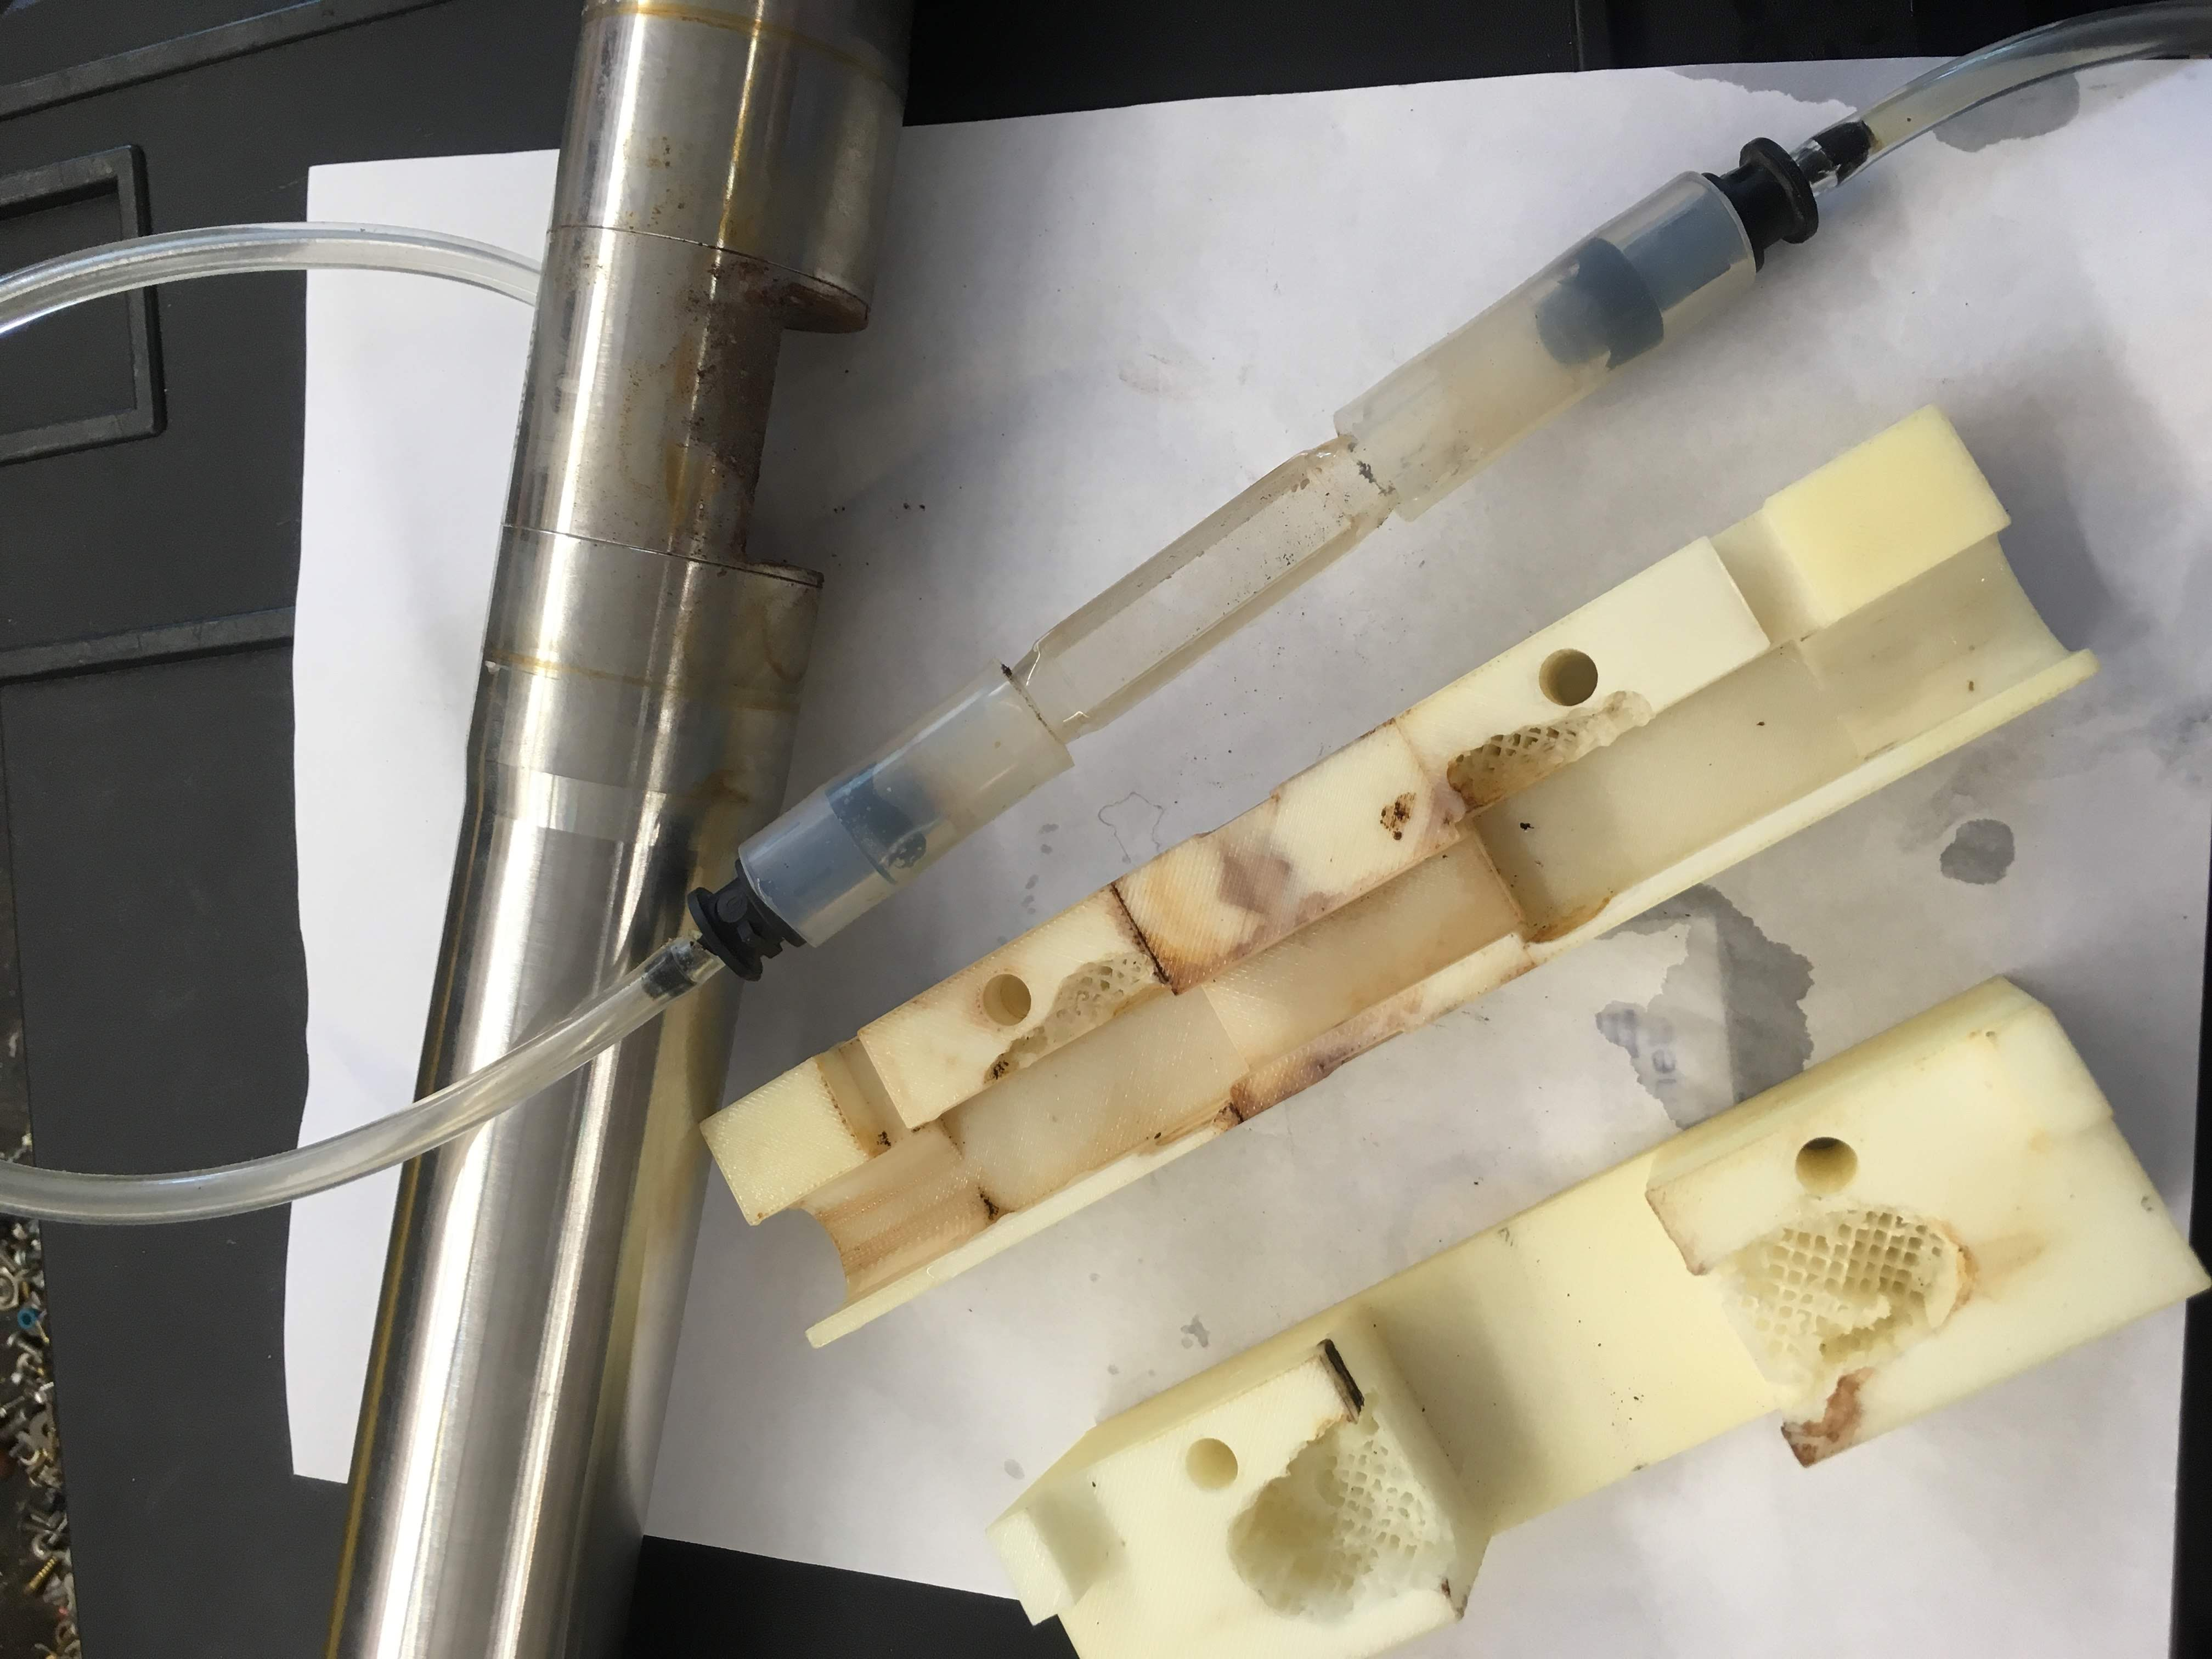
\includegraphics[width=0.8\linewidth]{pictures/Cuvette1} 

}

\caption{Flow through cuvette installed and its cuvette holder (not clean in the pictures here...)}\label{fig:Cuvette1}
\end{figure}

\begin{figure}

{\centering 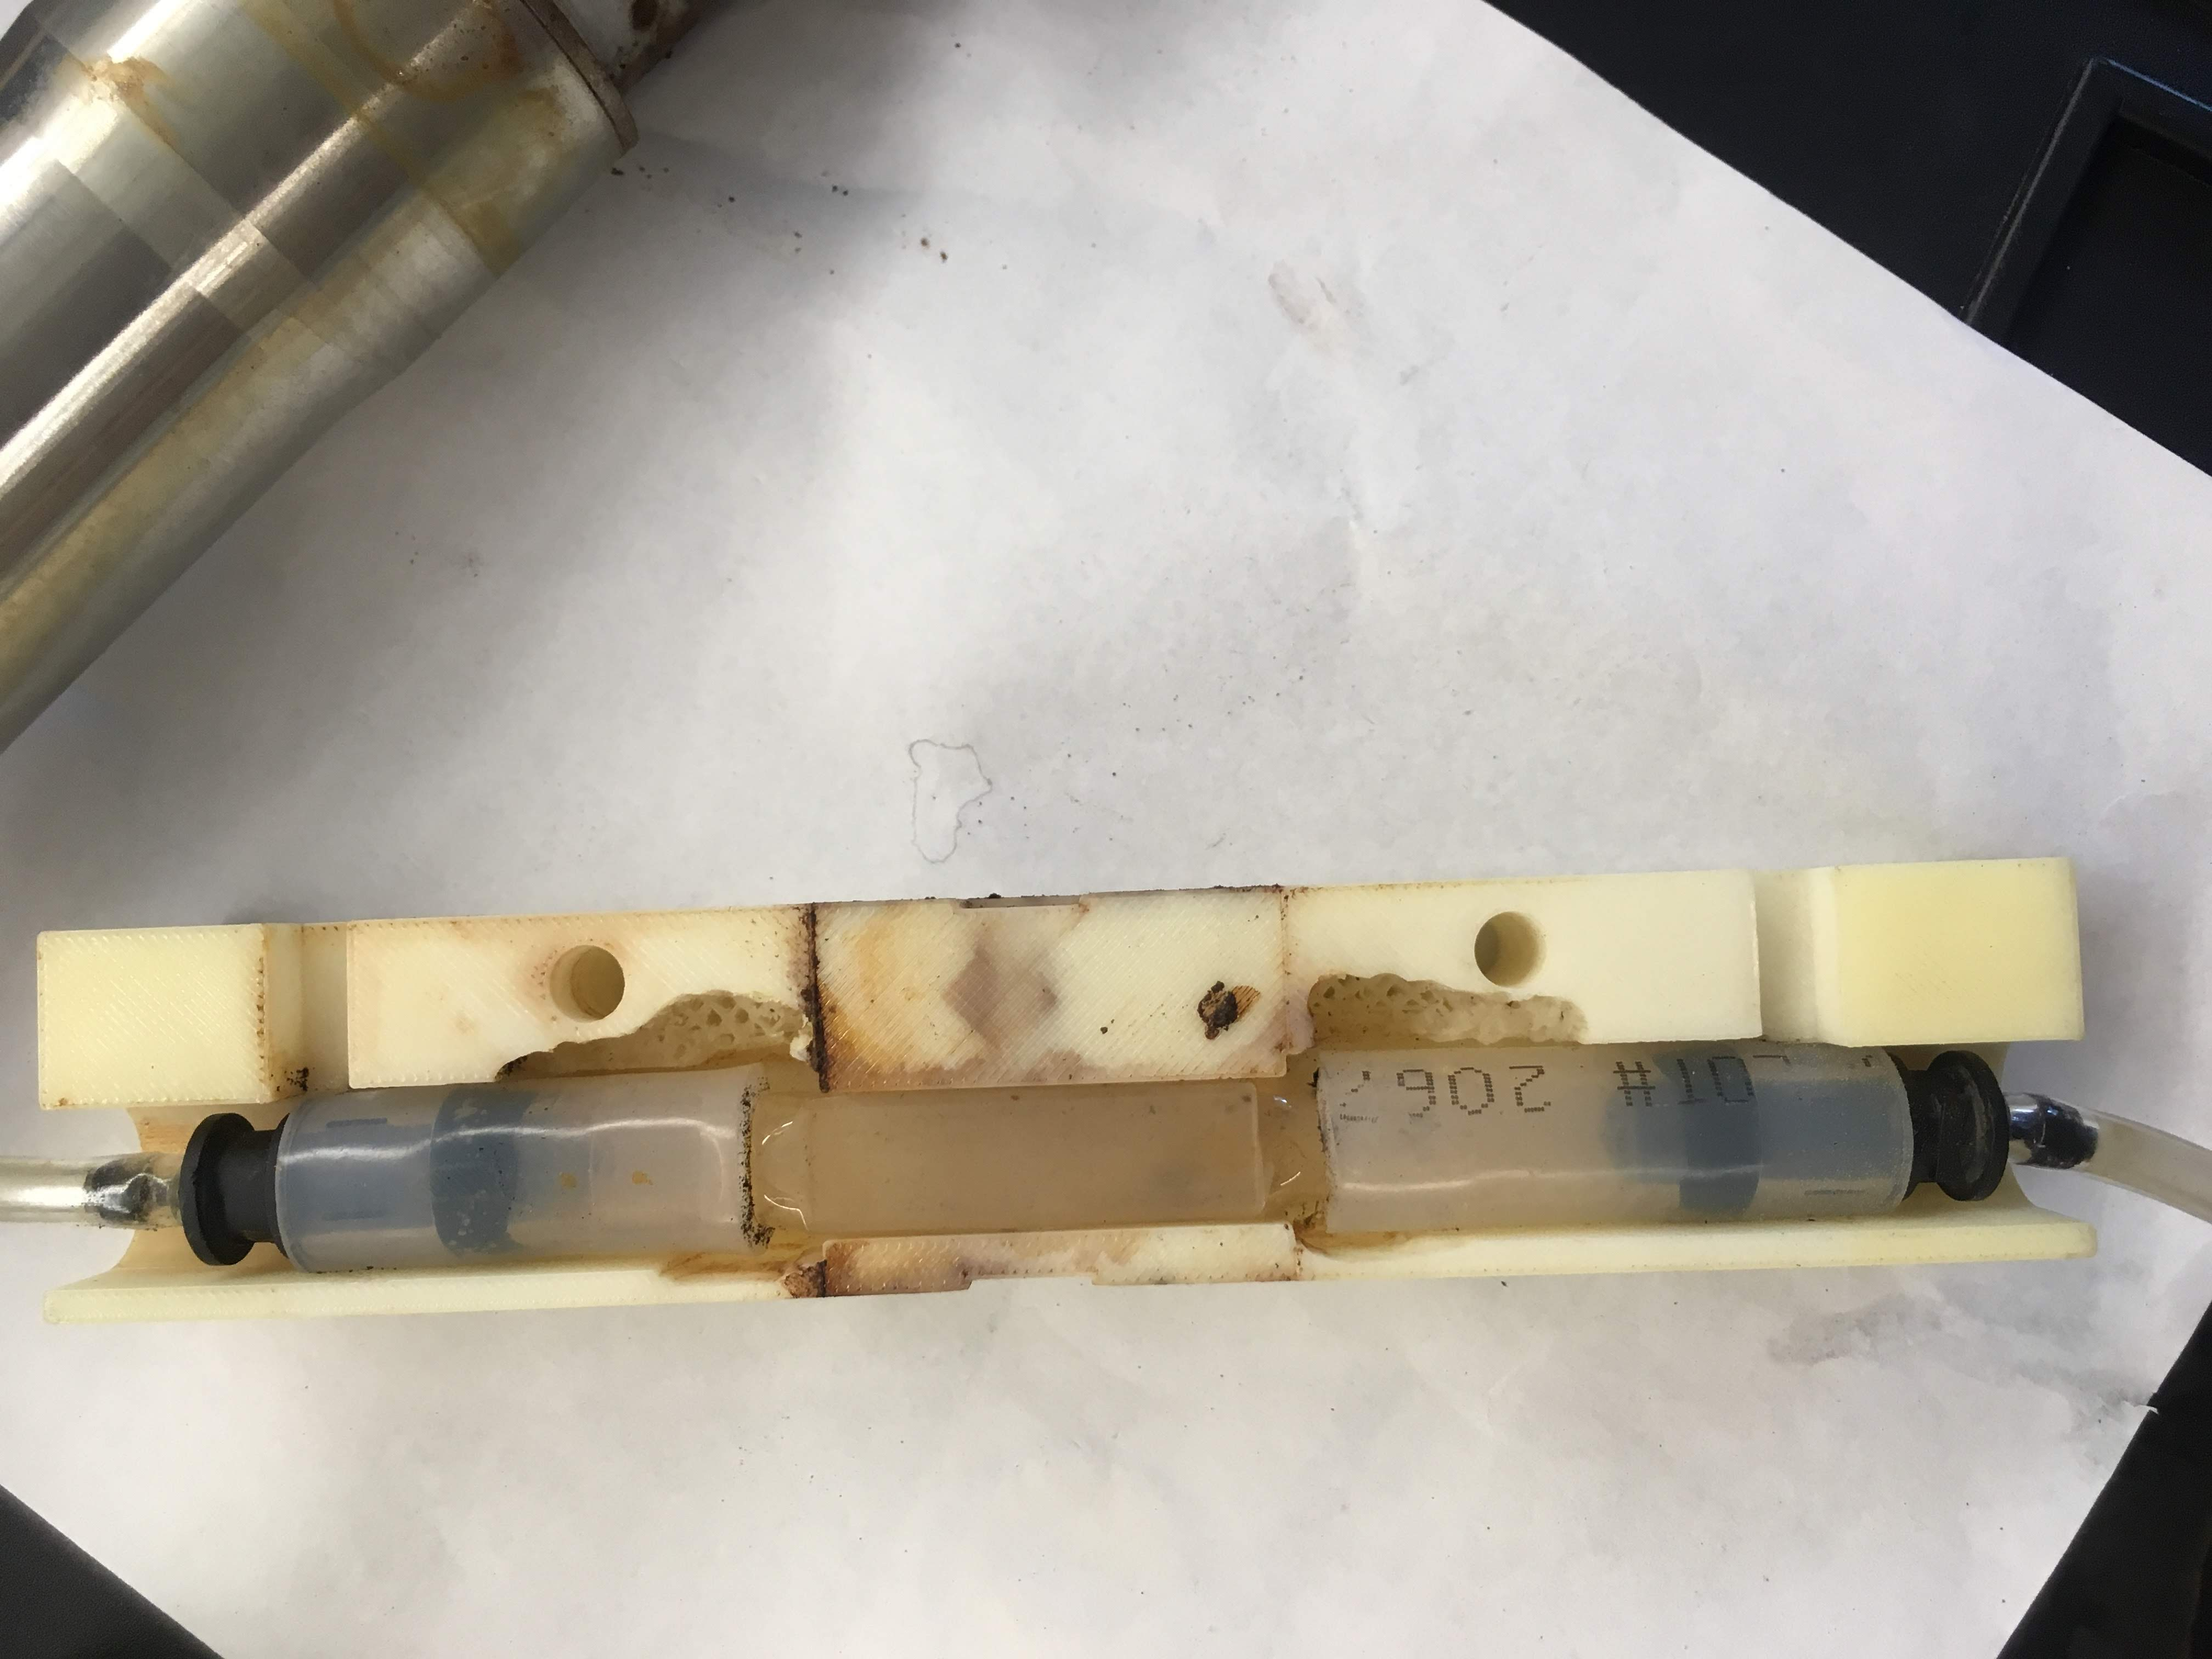
\includegraphics[width=0.8\linewidth]{pictures/Cuvette2} 

}

\caption{Flow through cuvette installed in its cuvette holder}\label{fig:Cuvette2}
\end{figure}

\begin{figure}

{\centering 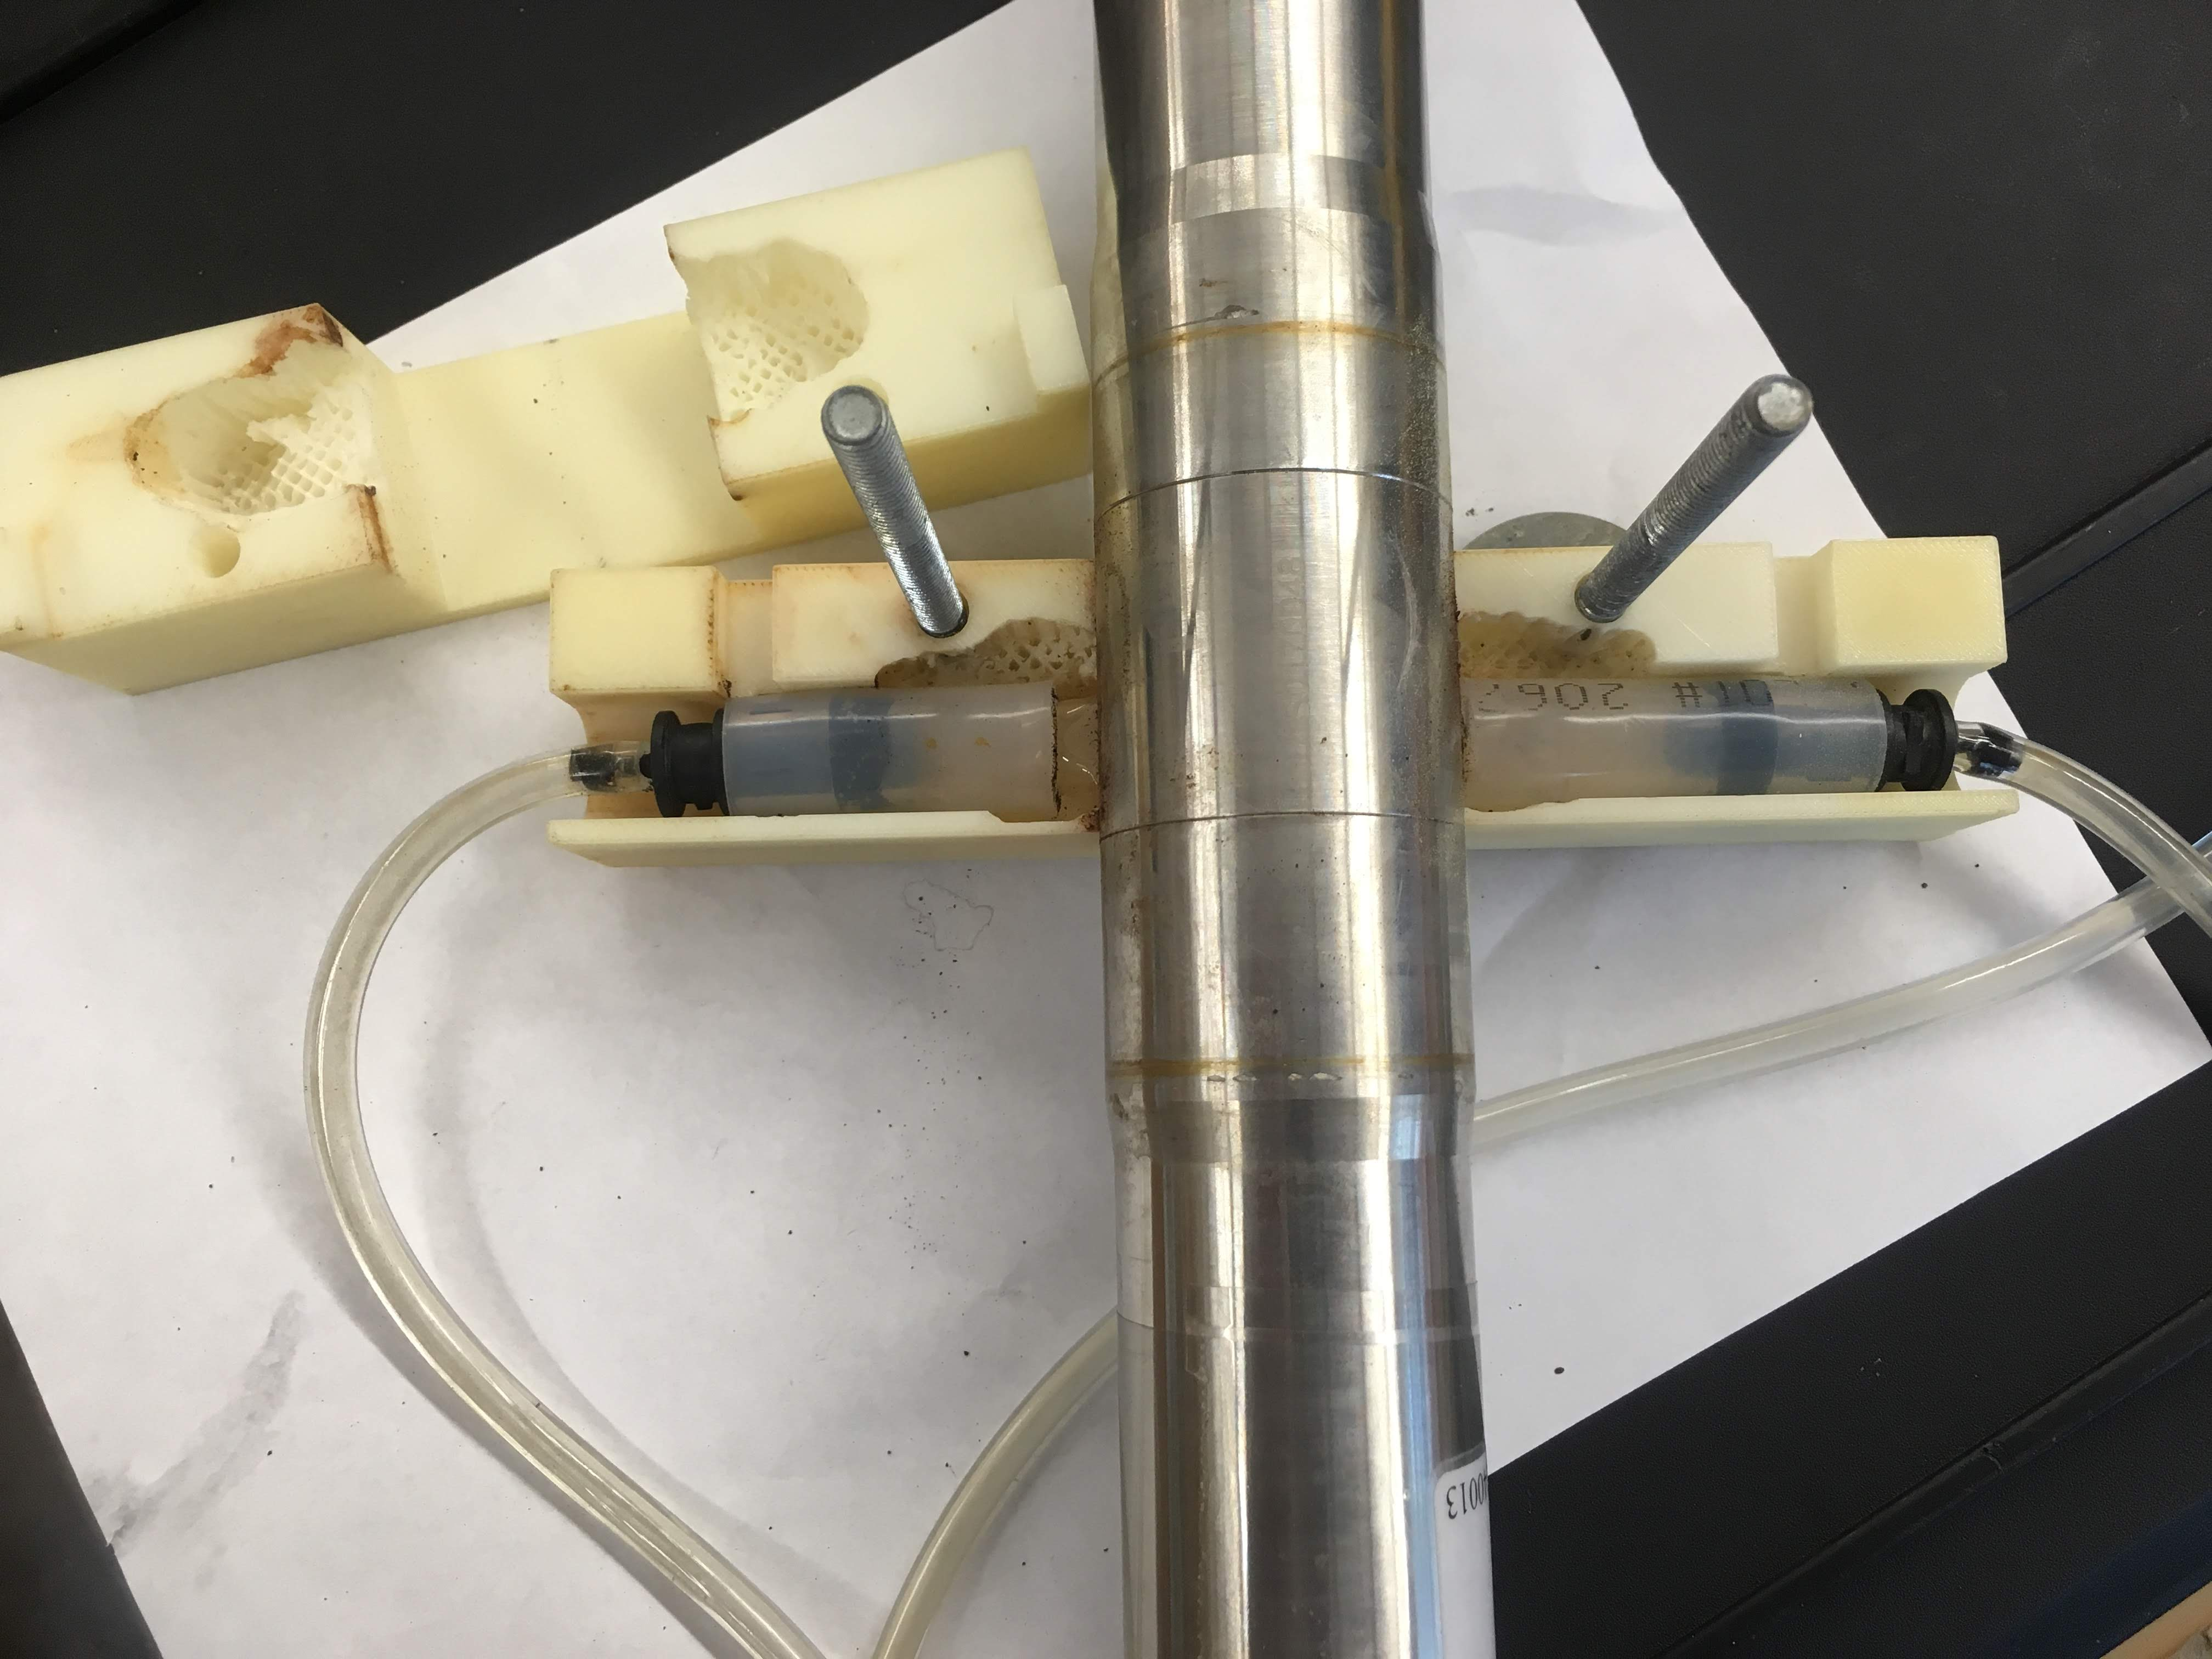
\includegraphics[width=0.8\linewidth]{pictures/CuvetteSpectro1} 

}

\caption{Flow through cuvette installed with the Spectro::lyser}\label{fig:CuvetteSpectro1}
\end{figure}

\begin{figure}

{\centering 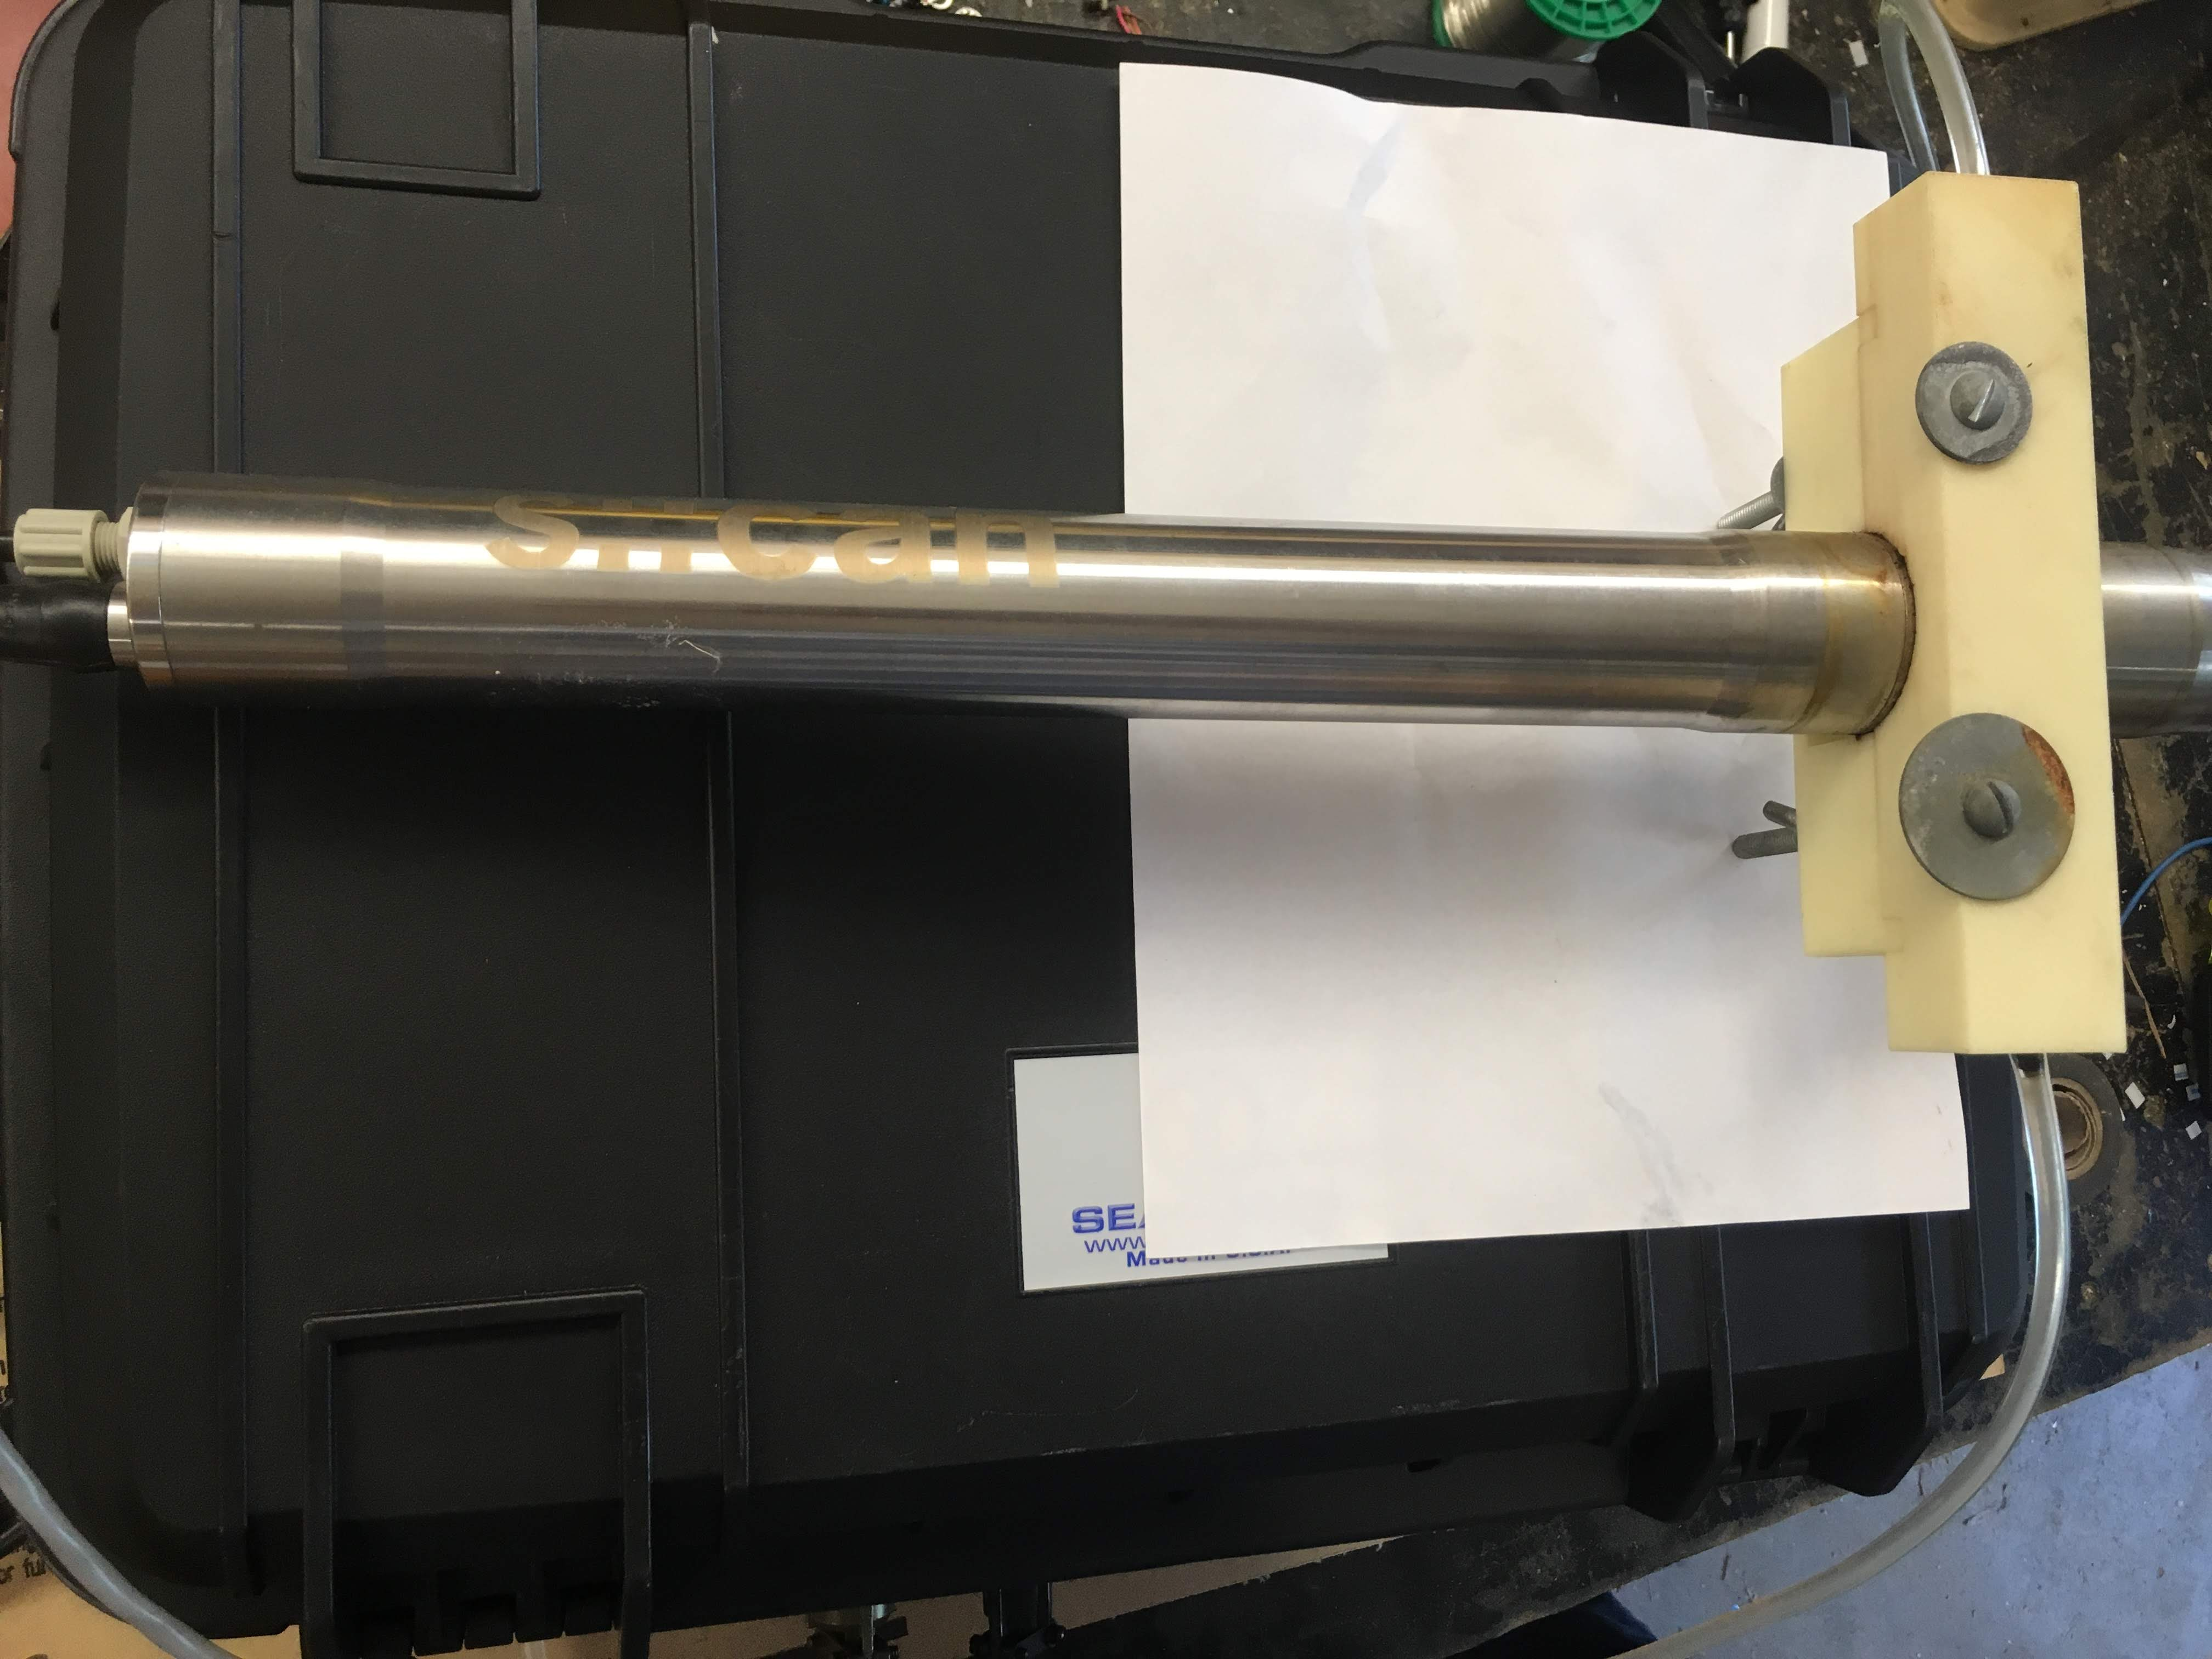
\includegraphics[width=0.8\linewidth]{pictures/CuvetteSpectro2} 

}

\caption{Full installation of the cuvette holder on the Spectro::lyser}\label{fig:CuvetteSpectro2}
\end{figure}

\hypertarget{configure-the-spectrolyser-for-cuvette}{%
\section{Configure the Spectro::lyser for cuvette}\label{configure-the-spectrolyser-for-cuvette}}

For this, you need to log on to your spectro::lyser as `Service' as illustrated below, and use the password \emph{Hermine}. Now, you need to be extremely careful at what you are doing at this point becaus any number you might change might affect the proper functioning of the instrument!

\begin{figure}

{\centering 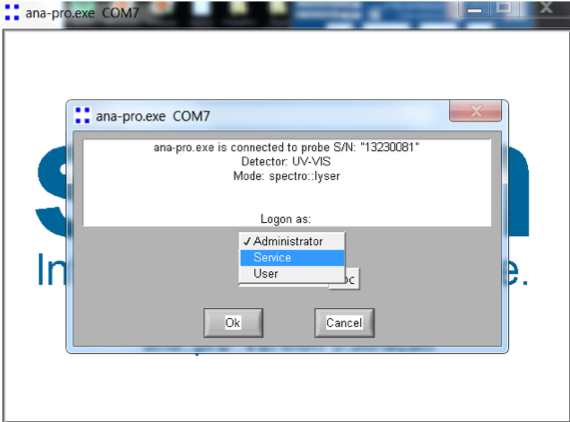
\includegraphics[width=0.7\linewidth]{pictures/SCAN-config-hermine} 

}

\caption{Log on the spectro::lyser as Service}\label{fig:SCAN-config-hermine}
\end{figure}

Now, go to Extra/Configuration as shown on the figure below.

\begin{figure}

{\centering 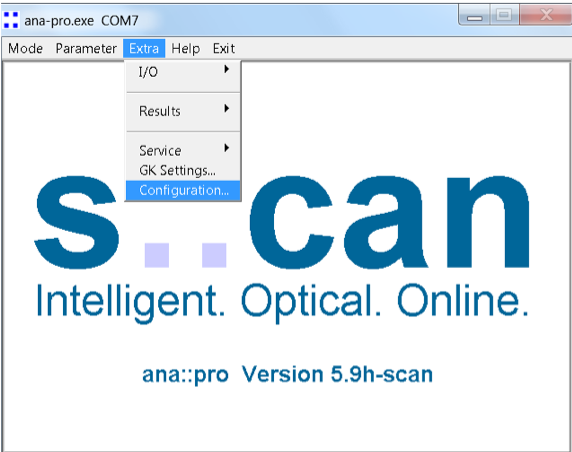
\includegraphics[width=0.7\linewidth]{pictures/SCAN-config-extra} 

}

\caption{Go to Extra/Configuration}\label{fig:SCAN-config-extra}
\end{figure}

This will take you to the core of where all the parameters of the spectro::lyser are stored. Again, this is a danger zone so be careful at what you modify or not. So there are two parameters that you can change here as a first step. Go on the top right corner of the screen and change the Path (highlighted in red ellipse) to ``Cuvette''. Now, the pathlength value is stored at the middle left of the screen (highlighted in red ellipse). You can see on the figure below that the value we have here is a 4 mm although we are actually using a 10 mm pathlenght cuvette. This is where it is a bit of an art and things are not fully clear from S::CAN. It is our understanding that the light bulb energy will automatically adjust to the `cuvette' mode and the pathlength we are giving it. This suggests that with lower pathlength values, the light energy should be adjusted lower since there is less `thickness' of water for light through which to travel. But we are not sure this always really works. In all cases, our experience has been that with the configuration used in the figure below, we have had good success in getting the `global calibration' to calculate reasonable nitrate and DOC concentrations. We therefore recommend to use this configuration as a starter. Should the global calibration still not calculate reasonable values, our suggestion is to use 0.01 m (or 10 mm) as pathlength.

\begin{figure}

{\centering 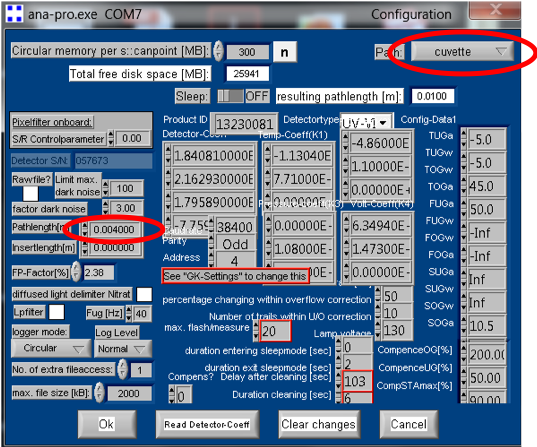
\includegraphics[width=0.7\linewidth]{pictures/SCAN-config-cuvette} 

}

\caption{Go to Extra/Configuration}\label{fig:SCAN-config-cuvette}
\end{figure}

Then log off and log back on as administrator.

\hypertarget{turn-the-mux-on}{%
\section{Turn the MUX on}\label{turn-the-mux-on}}

To turn the MUX on, put the top left swith to the \texttt{ON} position. When the Spectro::lyser is connected to the Con::nect box, the MUX starts its routine identifying a \emph{XXXX-MUX.txt} file, and then identifies a \emph{.fp} file. If the SD card is missing, there will be an NA file for the \emph{XXXX-MUX.txt} file. If the Spectro::lyser is not connected, there will be an NA file for the \emph{.fp} file. See video \ref{fig:TurnOnVideo} for illustration

\label{fig:TurnOnVideo}Illustration of initialization phase

\hypertarget{test-the-mux-in-the-lab}{%
\section{Test the MUX in the lab}\label{test-the-mux-in-the-lab}}

We recommend that before going out to the field, the user should test the MUX in the lab to get acquainted with the MUX, without having to deal with the field constraints. The contraption to connect the MUX the Spectro::lyser in the field should be tested in the lab first. It is also the time to build/test a sample spool.

It is the time to test the configuration the user is expected to have in the field. It is at that time to test the \emph{config.txt} file that is expected to be used. Only the pump times will have to be adjusted in the field afterwards. It is best to test the MUX over several days in the lab to get acquainted with the files generated on the SD card.

\hypertarget{install-and-test-the-mux-in-the-field}{%
\section{Install and test the MUX in the field}\label{install-and-test-the-mux-in-the-field}}

\hypertarget{install-all-hardware-to-length}{%
\subsection{Install all hardware to length}\label{install-all-hardware-to-length}}

When the lab tests have been successful, it is time to install the MUX-sensor system in the field with all the tubing cut to length. It is crucial that the final lengths be correct to test the proper \texttt{\textless{}PUMP\ TIMES\textgreater{}}, \texttt{\textless{}MEASUREMENT\ TIMES\textgreater{}}, and \texttt{\textless{}PURGE\ TIMES\textgreater{}}.

Make sure the intakes for all have screen or mesh size not larger than 1.2 mm. We have seen the pump stall because of large particles that got stuck in the peristaltic pump tubing.

\hypertarget{use-manual-pumping-feature-to-obtain-you-pump-and-purge-times}{%
\subsection{Use manual pumping feature to obtain you pump and purge times}\label{use-manual-pumping-feature-to-obtain-you-pump-and-purge-times}}

For that, the MUX has a \emph{manual pumping} and \emph{manual purging} feature. At the bottom right end of the control box, there is a toggle switch with three positions (Figure \ref{fig:ControlLabel1}): up for \texttt{FOR} or forward pumping, middle for neutral when not used in manual pumping mode, and down for \texttt{REV} or purging. Make sure you keep this toggle in neutral or middle position for all other use of the MUX.

\begin{figure}

{\centering 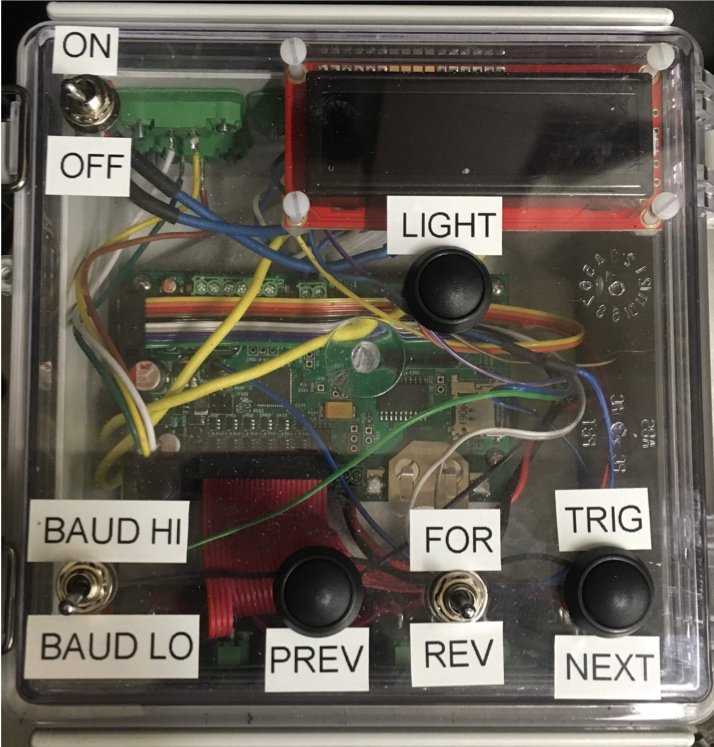
\includegraphics[width=0.6\linewidth]{pictures/ControlLabel} 

}

\caption{Control box panel display}\label{fig:ControlLabel1}
\end{figure}

When manual pumping or purging, a timer keeps track of time and gives the user an opportunity to time all the desired pumping and purging times, to be programed later in the \emph{config.txt} file. To switch from valve to valve, press the \texttt{PREV} button. An example is provided in the following video \ref{fig:ManualVideo}.

\label{fig:ManualVideo}Illustration of the manual pumping features

\hypertarget{manually-trigger-the-mux}{%
\subsection{Manually trigger the MUX}\label{manually-trigger-the-mux}}

Once you have recorded and implemented the timing in the field, it is time to trigger the MUX manually by pressing the \texttt{TRIG} button. A \emph{sampling sequence} will then start with the first valve on the \emph{config.txt} file. Adjust all timing accordingly and if needed after you observed how the \emph{sampling sequence} works.

\hypertarget{change-clock}{%
\subsection{Change clock}\label{change-clock}}

To change the clock, press together at the same time the \texttt{LIGHT}, \texttt{PREV}, and \texttt{NEXT} buttons. Advance on the screen using the \texttt{PREV}, and \texttt{NEXT} buttons. Change the values turning the switch up and down. The instructions are further illustrated on the video \ref{fig:ChangeClock}.

\label{fig:ChangeClock}Illustration of how to change the clock

\hypertarget{trouble-shooting}{%
\chapter{Trouble Shooting}\label{trouble-shooting}}

Still in construction.

\bibliography{book.bib,packages.bib}


\end{document}
